% generated by GAPDoc2LaTeX from XML source (Frank Luebeck)
\documentclass[a4paper,11pt]{report}

\usepackage{a4wide}
\sloppy
\pagestyle{myheadings}
\usepackage{amssymb}
\usepackage[latin1]{inputenc}
\usepackage{makeidx}
\makeindex
\usepackage{color}
\definecolor{FireBrick}{rgb}{0.5812,0.0074,0.0083}
\definecolor{RoyalBlue}{rgb}{0.0236,0.0894,0.6179}
\definecolor{RoyalGreen}{rgb}{0.0236,0.6179,0.0894}
\definecolor{RoyalRed}{rgb}{0.6179,0.0236,0.0894}
\definecolor{LightBlue}{rgb}{0.8544,0.9511,1.0000}
\definecolor{Black}{rgb}{0.0,0.0,0.0}

\definecolor{linkColor}{rgb}{0.0,0.0,0.554}
\definecolor{citeColor}{rgb}{0.0,0.0,0.554}
\definecolor{fileColor}{rgb}{0.0,0.0,0.554}
\definecolor{urlColor}{rgb}{0.0,0.0,0.554}
\definecolor{promptColor}{rgb}{0.0,0.0,0.589}
\definecolor{brkpromptColor}{rgb}{0.589,0.0,0.0}
\definecolor{gapinputColor}{rgb}{0.589,0.0,0.0}
\definecolor{gapoutputColor}{rgb}{0.0,0.0,0.0}

%%  for a long time these were red and blue by default,
%%  now black, but keep variables to overwrite
\definecolor{FuncColor}{rgb}{0.0,0.0,0.0}
%% strange name because of pdflatex bug:
\definecolor{Chapter }{rgb}{0.0,0.0,0.0}
\definecolor{DarkOlive}{rgb}{0.1047,0.2412,0.0064}


\usepackage{fancyvrb}

\usepackage{mathptmx,helvet}
\usepackage[T1]{fontenc}
\usepackage{textcomp}


\usepackage[
            pdftex=true,
            bookmarks=true,        
            a4paper=true,
            pdftitle={Written with GAPDoc},
            pdfcreator={LaTeX with hyperref package / GAPDoc},
            colorlinks=true,
            backref=page,
            breaklinks=true,
            linkcolor=linkColor,
            citecolor=citeColor,
            filecolor=fileColor,
            urlcolor=urlColor,
            pdfpagemode={UseNone}, 
           ]{hyperref}

\newcommand{\maintitlesize}{\fontsize{50}{55}\selectfont}

% write page numbers to a .pnr log file for online help
\newwrite\pagenrlog
\immediate\openout\pagenrlog =\jobname.pnr
\immediate\write\pagenrlog{PAGENRS := [}
\newcommand{\logpage}[1]{\protect\write\pagenrlog{#1, \thepage,}}
%% were never documented, give conflicts with some additional packages

\newcommand{\GAP}{\textsf{GAP}}

%% nicer description environments, allows long labels
\usepackage{enumitem}
\setdescription{style=nextline}

%% depth of toc
\setcounter{tocdepth}{1}



\usepackage{graphicx} \usepackage{float}

%% command for ColorPrompt style examples
\newcommand{\gapprompt}[1]{\color{promptColor}{\bfseries #1}}
\newcommand{\gapbrkprompt}[1]{\color{brkpromptColor}{\bfseries #1}}
\newcommand{\gapinput}[1]{\color{gapinputColor}{#1}}


\begin{document}

\logpage{[ 0, 0, 0 ]}
\begin{titlepage}
\mbox{}\vfill

\begin{center}{\maintitlesize \textbf{PatternClass\mbox{}}}\\
\vfill

\hypersetup{pdftitle=PatternClass}
\markright{\scriptsize \mbox{}\hfill PatternClass \hfill\mbox{}}
{\Huge \textbf{Permutation Pattern Classes\mbox{}}}\\
\vfill

{\Huge Version 1.12358\mbox{}}\\[1cm]
{February 2015\mbox{}}\\[1cm]
\mbox{}\\[2cm]
{\Large \textbf{Michael Albert \mbox{}}}\\
{\Large \textbf{Steve Linton \mbox{}}}\\
{\Large \textbf{Ruth Hoffmann \mbox{}}}\\
\hypersetup{pdfauthor=Michael Albert ; Steve Linton ; Ruth Hoffmann }
\end{center}\vfill

\mbox{}\\
{\mbox{}\\
\small \noindent \textbf{Michael Albert }  Email: \href{mailto:// malbert at cs.otago.ac.nz} {\texttt{ malbert at cs.otago.ac.nz}}}\\
{\mbox{}\\
\small \noindent \textbf{Steve Linton }  Email: \href{mailto:// sl4 at st-andrews.ac.uk} {\texttt{ sl4 at st-andrews.ac.uk}}}\\
{\mbox{}\\
\small \noindent \textbf{Ruth Hoffmann }  Email: \href{mailto:// rh347 at st-andrews.ac.uk} {\texttt{ rh347 at st-andrews.ac.uk}}}\\
\end{titlepage}

\newpage\setcounter{page}{2}
{\small 
\section*{Abstract}
\logpage{[ 0, 0, 1 ]}
 The \texttt{PatternClass} package is build on the idea of token passing networks building permutation
pattern classes. Those classes are best determined by their basis. Both sets
can be encoded by rank encoding their permutations. Each, the class and its
basis, in their encoded form build a rational language \cite{RegCloSetPerms}. Rational languages can be easily computed by using automata, which also can
be build directly from the token passing networks \cite{PermGenTPGraph}. Both ways will build the same language, i.e. the same automaton. \mbox{}}\\[1cm]
{\small 
\section*{Copyright}
\logpage{[ 0, 0, 2 ]}
{\copyright} 2011 by Michael Albert, Steve Linton and Ruth Hoffmann\mbox{}}\\[1cm]
\newpage

\def\contentsname{Contents\logpage{[ 0, 0, 3 ]}}

\tableofcontents
\newpage

 
\chapter{\textcolor{Chapter }{Introduction}}\logpage{[ 1, 0, 0 ]}
\hyperdef{L}{X7DFB63A97E67C0A1}{}
{
 Token passing networks (TPNs) are directed graphs with nodes that can hold at
most one token. Also each graph has a designated input node, which generates
an ordered sequence of numbered tokens and a designated output node that
collects the tokens in the order they arrive at it. The input node has no
incoming edges, whereas the output node has no outgoing edges. A token $t$ travels through the graph, from node to node, if there is an edge connecting
the nodes, if the node the token is moving from is either the input node and
the tokens $1, \ldots, t-1$ have been released or the node is not the output node, and lastly if the
destination node contains no token or it is the output node. \cite{PermGenTPGraph} 

 The set of permutations resulting from a TPN is closed under the property of
containment. A permutation $a$ contains a permutation $b$ of shorter length if in $a$ there is a subsequence that is isomorphic to $b$. This class of permutations can be represented by its anti-chain, which in
this context is called the basis. \cite{RegCloSetPerms} 

 To enhance the computability of permutation pattern classes, each permutation
can be encoded, using the so called rank encoding. For a permutation $p_{1} \ldots p_{n}$, it is the sequence $e_{1}\ldots e_{n}$ where $e_{i}$ is the rank of $p_{i}$ among $\{p_{i},p_{i+1},\ldots,p_{n}\}$. It can be shown that the sets of encoded permutations of the class and the
basis, both are a rational languages. Rational languages can be represented by
automata. \cite{RegCloSetPerms} 

 There is another approach to get from TPNs to their corresponding automata.
Namely building equivalence classes from TPNs using the different dispositions
of tokens within them. These equivalence classes of dispositions and the rank
encoding of the permutations allow to build the same rational language as from
the process above. \cite{PermGenTPGraph} }

 
\chapter{\textcolor{Chapter }{Token Passing Networks}}\logpage{[ 2, 0, 0 ]}
\hyperdef{L}{X7C769071875E96B2}{}
{
 \label{tpn} A token passing network is a directed graph with a designated input node and a
designated output node. The input node has no incoming edges whereas the
output node has no outgoing edges. Also the input node generates a sequence of
tokens, labelled 1, 2, 3, ... . These tokens are passed on to the nodes within
the graph, where each node, apart from the input and output node, can hold at
most one token at any time. The edges do not hold tokens but are there to pass
them on. The following must hold if a token $t$ moves from the node $x$ to the node $y$. 

 There is an edge from $x$ to $y$; $x$ is the input node, and the tokens 1, 2, 3, ... , $t-1$ have been moved, or $x$ is any other node but not the output node; lastly either $y$ is the output node or $y$ is not the input node and currently is not occupied by a token. \cite{PermGenTPGraph} 

 Token passing networks, or TPNs, are represented in \textsf{GAP} as a list. Each entry of the list is the index of the node within the TPN and
contains a list of the "destinations", i.e. the end of the edge or arrow where
it is directed to. 

 Here is an example how the input of such a TPN looks in \textsf{GAP}: 
\begin{Verbatim}[commandchars=!@|,fontsize=\small,frame=single,label=Example]
  !gapprompt@gap>| !gapinput@hex:=[[2,3],[4],[5],[3,6],[6],[]];|
  [ [ 2, 3 ], [ 4 ], [ 5 ], [ 3, 6 ], [ 6 ], [  ] ]
  !gapprompt@gap>| !gapinput@|
\end{Verbatim}
  This list represents the following directed graph: \begin{figure}[H]
\begin{center} \leavevmode 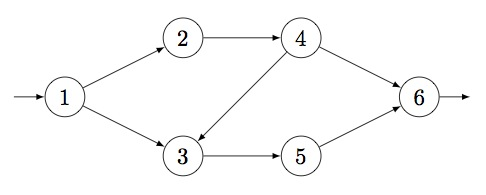
\includegraphics[scale=0.75]{img/hex.jpg}
\end{center} \end{figure}   From this it is visible that the input node is 1, as it has no other node
pointing any arrows towards it, and the output node is 6, as it has no
destinations (hence the empty list). 
\section{\textcolor{Chapter }{ Specific TPN }}\logpage{[ 2, 1, 0 ]}
\hyperdef{L}{X80EE110279808BD3}{}
{
 In \texttt{PatternClass} there are several functions that define different kinds of specific token
passing networks. 

\subsection{\textcolor{Chapter }{Parstacks}}
\logpage{[ 2, 1, 1 ]}\nobreak
\hyperdef{L}{X85AFF5537F917AEB}{}
{\noindent\textcolor{FuncColor}{$\triangleright$\ \ \texttt{Parstacks({\mdseries\slshape m, n})\index{Parstacks@\texttt{Parstacks}}
\label{Parstacks}
}\hfill{\scriptsize (function)}}\\
\textbf{\indent Returns:\ }
A list that represents the directed edges of a token passing network.



 \texttt{Parstacks} constructs a token passing network with 2 different sized stacks \texttt{m,n} positioned in parallel. 
\begin{Verbatim}[commandchars=!@|,fontsize=\small,frame=single,label=Example]
  !gapprompt@gap>| !gapinput@Parstacks(2,2);|
  [ [ 2, 4 ], [ 3, 6 ], [ 2 ], [ 5, 6 ], [ 4 ], [  ] ]
  !gapprompt@gap>| !gapinput@|
\end{Verbatim}
  \texttt{Parstacks(2,2)} can be visualised as the following directed graph: \begin{figure}[H]
\begin{center} \leavevmode 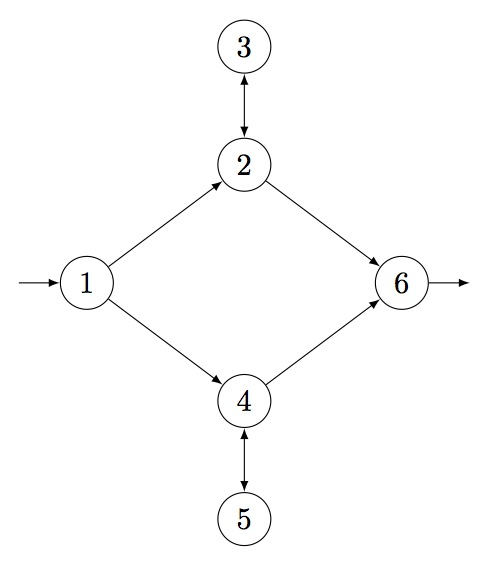
\includegraphics[scale=0.75]{img/ps22.jpg}
\end{center} \end{figure}   
\begin{Verbatim}[commandchars=!@|,fontsize=\small,frame=single,label=Example]
  !gapprompt@gap>| !gapinput@Parstacks(4,3);|
  [ [ 2, 6 ], [ 3, 9 ], [ 2, 4 ], [ 3, 5 ], [ 4 ], [ 7, 9 ], [ 6, 8 ], [ 7 ],
    [  ] ]
  !gapprompt@gap>| !gapinput@|
\end{Verbatim}
  The token passing network below represents the list that was output by \texttt{Parstacks(4,3)}. \begin{figure}[H] \begin{center} \leavevmode
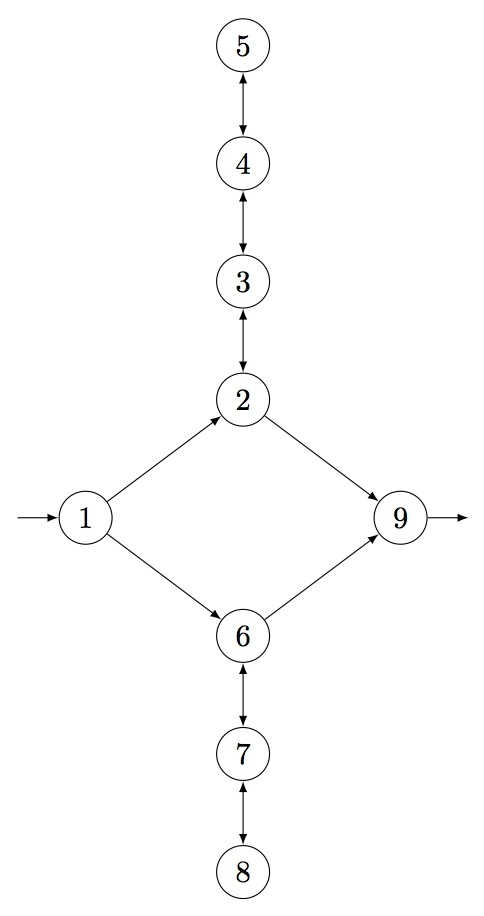
\includegraphics[scale=0.75]{img/ps43.jpg} \end{center} \end{figure}   }

 

\subsection{\textcolor{Chapter }{Seqstacks}}
\logpage{[ 2, 1, 2 ]}\nobreak
\hyperdef{L}{X7D6D07D980634845}{}
{\noindent\textcolor{FuncColor}{$\triangleright$\ \ \texttt{Seqstacks({\mdseries\slshape n[, m[, o[, p[, ...]]]]})\index{Seqstacks@\texttt{Seqstacks}}
\label{Seqstacks}
}\hfill{\scriptsize (function)}}\\
\textbf{\indent Returns:\ }
A list that represents the directed edges of a token passing network.



 The token passing network build by \texttt{Seqstacks} contains a series of stacks (as many as you have integers in the arguments
list) each of different length (each integer in the argument list). 
\begin{Verbatim}[commandchars=!@|,fontsize=\small,frame=single,label=Example]
  !gapprompt@gap>| !gapinput@Seqstacks(2,2);|
  [ [ 2 ], [ 3, 4 ], [ 2 ], [ 5, 6 ], [ 4 ], [  ] ]
  !gapprompt@gap>| !gapinput@|
\end{Verbatim}
  \texttt{Seqstacks(2,2)} can be visualised as the following directed graph: \begin{figure}[H]
\begin{center} \leavevmode 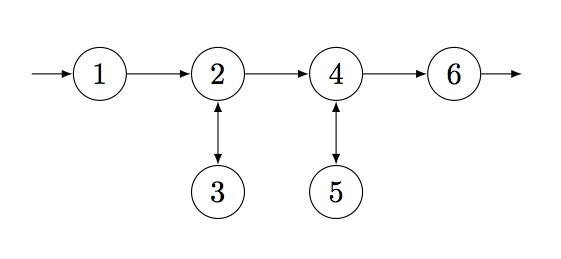
\includegraphics[scale=0.75]{img/ss22.jpg}
\end{center} \end{figure}   
\begin{Verbatim}[commandchars=!@|,fontsize=\small,frame=single,label=Example]
  !gapprompt@gap>| !gapinput@Seqstacks(3,1,4);|
  [ [ 2 ], [ 3, 5 ], [ 2, 4 ], [ 3 ], [ 4 ], [ 7, 10 ], [ 6, 8 ], [ 7, 9 ], 
    [ 8 ], [  ] ]
  !gapprompt@gap>| !gapinput@|
\end{Verbatim}
  The token passing network containing a series of stacks of length 3, 1 and 4
looks as follows: \begin{figure}[H] \begin{center} \leavevmode
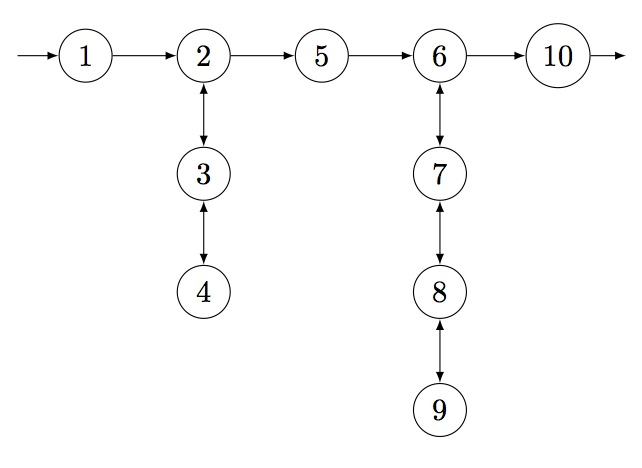
\includegraphics[scale=0.75]{img/ss314.jpg} \end{center} \end{figure}   }

 

\subsection{\textcolor{Chapter }{BufferAndStack}}
\logpage{[ 2, 1, 3 ]}\nobreak
\hyperdef{L}{X81E3656E85CB6EB7}{}
{\noindent\textcolor{FuncColor}{$\triangleright$\ \ \texttt{BufferAndStack({\mdseries\slshape m, n})\index{BufferAndStack@\texttt{BufferAndStack}}
\label{BufferAndStack}
}\hfill{\scriptsize (function)}}\\
\textbf{\indent Returns:\ }
A list that represents the directed edges of a token passing network.



 \texttt{BufferAndStack} is a token passing network that consists of a buffer of size \texttt{m} which is followed by a single stack of size \texttt{n}. 
\begin{Verbatim}[commandchars=!@|,fontsize=\small,frame=single,label=Example]
  !gapprompt@gap>| !gapinput@BufferAndStack(2,2);|
  [ [ 2, 3 ], [ 4 ], [ 4 ], [ 5, 6 ], [ 4 ], [  ] ]
  !gapprompt@gap>| !gapinput@|
\end{Verbatim}
  \texttt{BufferAndStack(2,2)} is the following directed graph: \begin{figure}[H] \begin{center} \leavevmode
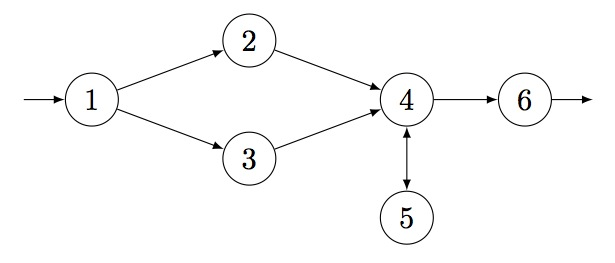
\includegraphics[scale=0.75]{img/bs22.jpg} \end{center} \end{figure}   
\begin{Verbatim}[commandchars=!@|,fontsize=\small,frame=single,label=Example]
  !gapprompt@gap>| !gapinput@BufferAndStack(4,3);|
  [ [ 2 .. 5 ], [ 6 ], [ 6 ], [ 6 ], [ 6 ], [ 7, 9 ], [ 6, 8 ], [ 7 ], [  ] ]
  !gapprompt@gap>| !gapinput@|
\end{Verbatim}
  The token passing network correlating to the list output by \texttt{BufferAndStack(4,3)} is: \begin{figure}[H] \begin{center} \leavevmode
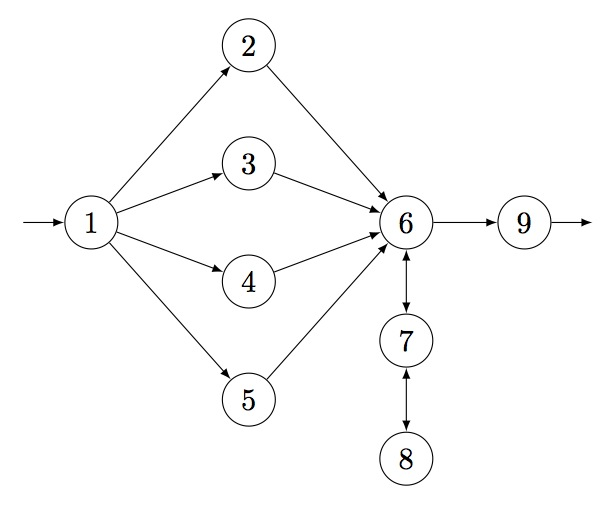
\includegraphics[scale=0.75]{img/bs43.jpg} \end{center} \end{figure}   }

 }

 }

 
\chapter{\textcolor{Chapter }{Permutation Encoding}}\logpage{[ 3, 0, 0 ]}
\hyperdef{L}{X8696E21E80C1AEC1}{}
{
 A permutation $\pi=\pi_{1} \ldots \pi_{n}$ has rank encoding $p_{1} \ldots p_{n}$ where $ p_{i}= |\{j : j \geq i, \pi_{j} \leq \pi_{i} \} | $. In other words the rank encoded permutation is a sequence of $p_{i}$ with $1\leq i\leq n$, where $p_{i}$ is the rank of $\pi_{i}$ in $\{\pi_{i},\pi_{i+1},\ldots ,\pi_{n}\}$. \cite{RegCloSetPerms} 

 The encoding of the permutation 3 2 5 1 6 7 4 8 9 is done as follows: \begin{center}
\begin{tabular}{c|c|c}Permutation&
Encoding&
Assisting list\\
325167489&
$\emptyset$&
123456789\\
25167489&
3&
12456789\\
5167489&
32&
1456789\\
167489&
323&
146789\\
67489&
3231&
46789\\
7489&
32312&
4789\\
489&
323122&
489\\
89&
3231221&
89\\
9&
32312211&
9\\
$\emptyset$&
323122111&
$\emptyset$\\
\end{tabular}\\[2mm]
\end{center}

 Decoding a permutation is done in a similar fashion, taking the sequence $p_{1} \ldots p_{n}$ and using the reverse process will lead to the permutation $\pi=\pi_{1} \ldots \pi_{n}$, where $\pi_{i}$ is determined by finding the number that has rank $p_{i}$ in $\{\pi_{i}, \pi_{i+1}, \ldots , \pi_{n}\}$. 

 The sequence 3 2 3 1 2 2 1 1 1 is decoded as: \begin{center}
\begin{tabular}{c|c|c}Encoding&
Permutation&
Assisting list\\
323122111&
$\emptyset$&
123456789\\
23122111&
3&
12456789\\
3122111&
32&
1456789\\
122111&
325&
146789\\
22111&
3251&
46789\\
2111&
32516&
4789\\
111&
325167&
489\\
11&
3251674&
89\\
1&
32516748&
9\\
$\emptyset$&
325167489&
$\emptyset$\\
\end{tabular}\\[2mm]
\end{center}

 
\section{\textcolor{Chapter }{ Encoding and Decoding }}\logpage{[ 3, 1, 0 ]}
\hyperdef{L}{X793F8BF48048365F}{}
{
 

\subsection{\textcolor{Chapter }{RankEncoding}}
\logpage{[ 3, 1, 1 ]}\nobreak
\hyperdef{L}{X8143AF3D79F4CC1D}{}
{\noindent\textcolor{FuncColor}{$\triangleright$\ \ \texttt{RankEncoding({\mdseries\slshape p})\index{RankEncoding@\texttt{RankEncoding}}
\label{RankEncoding}
}\hfill{\scriptsize (function)}}\\
\textbf{\indent Returns:\ }
A list that represents the rank encoding of the permutation \texttt{p}. 



 Using the algorithm above \texttt{RankEncoding} turns the permutation \texttt{p} into a list of integers. 
\begin{Verbatim}[commandchars=!@|,fontsize=\small,frame=single,label=Example]
  !gapprompt@gap>| !gapinput@RankEncoding([3, 2, 5, 1, 6, 7, 4, 8, 9]);|
  [ 3, 2, 3, 1, 2, 2, 1, 1, 1 ]
  !gapprompt@gap>| !gapinput@RankEncoding([ 4, 2, 3, 5, 1 ]);                 |
  [ 4, 2, 2, 2, 1 ]
  !gapprompt@gap>| !gapinput@|
\end{Verbatim}
 }

 

\subsection{\textcolor{Chapter }{RankDecoding}}
\logpage{[ 3, 1, 2 ]}\nobreak
\hyperdef{L}{X7DA97A7B7C8EB18A}{}
{\noindent\textcolor{FuncColor}{$\triangleright$\ \ \texttt{RankDecoding({\mdseries\slshape e})\index{RankDecoding@\texttt{RankDecoding}}
\label{RankDecoding}
}\hfill{\scriptsize (function)}}\\
\textbf{\indent Returns:\ }
A permutation in list form.



 A rank encoded permutation is decoded by using the reversed process from
encoding, which is also explained above. 
\begin{Verbatim}[commandchars=!@|,fontsize=\small,frame=single,label=Example]
  !gapprompt@gap>| !gapinput@RankDecoding([ 3, 2, 3, 1, 2, 2, 1, 1, 1 ]);|
  [ 3, 2, 5, 1, 6, 7, 4, 8, 9 ]
  !gapprompt@gap>| !gapinput@RankDecoding([ 4, 2, 2, 2, 1 ]);|
  [ 4, 2, 3, 5, 1 ]
  !gapprompt@gap>| !gapinput@|
\end{Verbatim}
 }

 

\subsection{\textcolor{Chapter }{SequencesToRatExp}}
\logpage{[ 3, 1, 3 ]}\nobreak
\hyperdef{L}{X832A1FEC7E5491EA}{}
{\noindent\textcolor{FuncColor}{$\triangleright$\ \ \texttt{SequencesToRatExp({\mdseries\slshape list})\index{SequencesToRatExp@\texttt{SequencesToRatExp}}
\label{SequencesToRatExp}
}\hfill{\scriptsize (function)}}\\
\textbf{\indent Returns:\ }
A rational expression that describes all the words in \texttt{list}.



 A list of sequences is turned into a rational expression by concatenating each
sequence and unifying all of them. 
\begin{Verbatim}[commandchars=!@|,fontsize=\small,frame=single,label=Example]
  !gapprompt@gap>| !gapinput@SequencesToRatExp([[ 1, 1, 1, 1, 1 ],[ 2, 1, 2, 2, 1 ],[ 3, 2, 1, 2, 1 ],|
  !gapprompt@>| !gapinput@[ 4, 2, 3, 2, 1 ]]);|
  11111U21221U32121U42321
  !gapprompt@gap>| !gapinput@|
\end{Verbatim}
 }

 }

 }

 
\chapter{\textcolor{Chapter }{From Networks to Automata}}\logpage{[ 4, 0, 0 ]}
\hyperdef{L}{X84E9957A81BF938D}{}
{
 It is known that the language of all encoded permutations of a TPN is
rational, and thus is it indeed possible to turn a TPN into an automaton. The
idea is to inspect all dispositions of tokens within the TPN and find
equivalence classes of these dispositions, for more details consult \cite{PermGenTPGraph}. Adding a constraint, which limits the number of tokens at any time within
the TPN, is also considered in this chapter. 

 The algorithms featured in this chapter do not return the minimal automata
representing the input TPN as they are exactly visualising the equivalence
classes of the dispositions of the tokens in the TPN. The automaton can be
minimalised by choice, as it simplifies future computations involving the
automaton also is makes the automata more legible. 
\section{\textcolor{Chapter }{Functions}}\logpage{[ 4, 1, 0 ]}
\hyperdef{L}{X86FA580F8055B274}{}
{
 

\subsection{\textcolor{Chapter }{GraphToAut}}
\logpage{[ 4, 1, 1 ]}\nobreak
\hyperdef{L}{X7CFD21C47E43D8FF}{}
{\noindent\textcolor{FuncColor}{$\triangleright$\ \ \texttt{GraphToAut({\mdseries\slshape g, innode, outnode})\index{GraphToAut@\texttt{GraphToAut}}
\label{GraphToAut}
}\hfill{\scriptsize (function)}}\\
\textbf{\indent Returns:\ }
An automaton representing the input TPN.



 \texttt{GraphToAut} turns an array represented directed graph, with a distinct input node and a
distinct output node, into the corresponding automaton, that accepts the
language build by the resulting rank encoded permutations of the directed
graph. 
\begin{Verbatim}[commandchars=!@B,fontsize=\small,frame=single,label=Example]
  !gapprompt@gap>B !gapinput@x:=Seqstacks(2,2);B
  [ [ 2 ], [ 3, 4 ], [ 2 ], [ 5, 6 ], [ 4 ], [  ] ]
  !gapprompt@gap>B !gapinput@aut:=GraphToAut(x,1,6);B
  < epsilon automaton on 4 letters with 64 states >
  !gapprompt@gap>B !gapinput@aut:=MinimalAutomaton(aut);B
  < deterministic automaton on 3 letters with 3 states >
  !gapprompt@gap>B !gapinput@Display(aut);B
     |  1  2  3  
  --------------
   a |  1  3  1  
   b |  3  3  3  
   c |  2  2  2  
  Initial state:   [ 1 ]
  Accepting state: [ 1 ]
  !gapprompt@gap>B !gapinput@B
\end{Verbatim}
  The minimal automaton corresponding to \texttt{Seqstacks(2,2)} is: \begin{figure}[H] \begin{center} \leavevmode
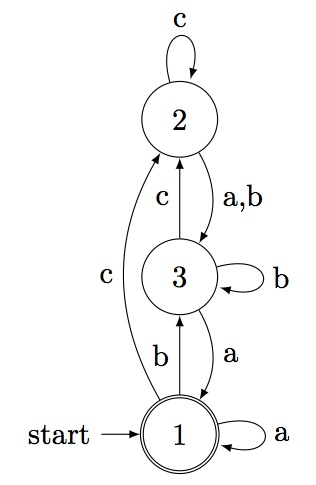
\includegraphics[scale=0.75]{img/ss22aut.jpg} \end{center} \end{figure}   
\begin{Verbatim}[commandchars=!@B,fontsize=\small,frame=single,label=Example]
  !gapprompt@gap>B !gapinput@x:=Parstacks(2,2);B
  [ [ 2, 4 ], [ 3, 6 ], [ 2 ], [ 5, 6 ], [ 4 ], [  ] ]
  !gapprompt@gap>B !gapinput@aut:=GraphToAut(x,1,6);B
  < epsilon automaton on 5 letters with 66 states >
  !gapprompt@gap>B !gapinput@aut:=MinimalAutomaton(aut);B
  < deterministic automaton on 4 letters with 9 states >
  !gapprompt@gap>B !gapinput@Display(aut);B
     |  1  2  3  4  5  6  7  8  9  
  --------------------------------
   a |  1  2  1  3  2  2  6  6  3  
   b |  3  2  3  3  4  3  6  9  3  
   c |  9  2  9  4  6  6  4  9  9  
   d |  8  2  8  7  5  5  7  8  8  
  Initial state:   [ 1 ]
  Accepting state: [ 1 ]
  !gapprompt@gap>B !gapinput@B
\end{Verbatim}
  The rank encoded permutations of \texttt{Parstacks(2,2)} are accepted by the following automaton: \begin{figure}[H] \begin{center}
\leavevmode 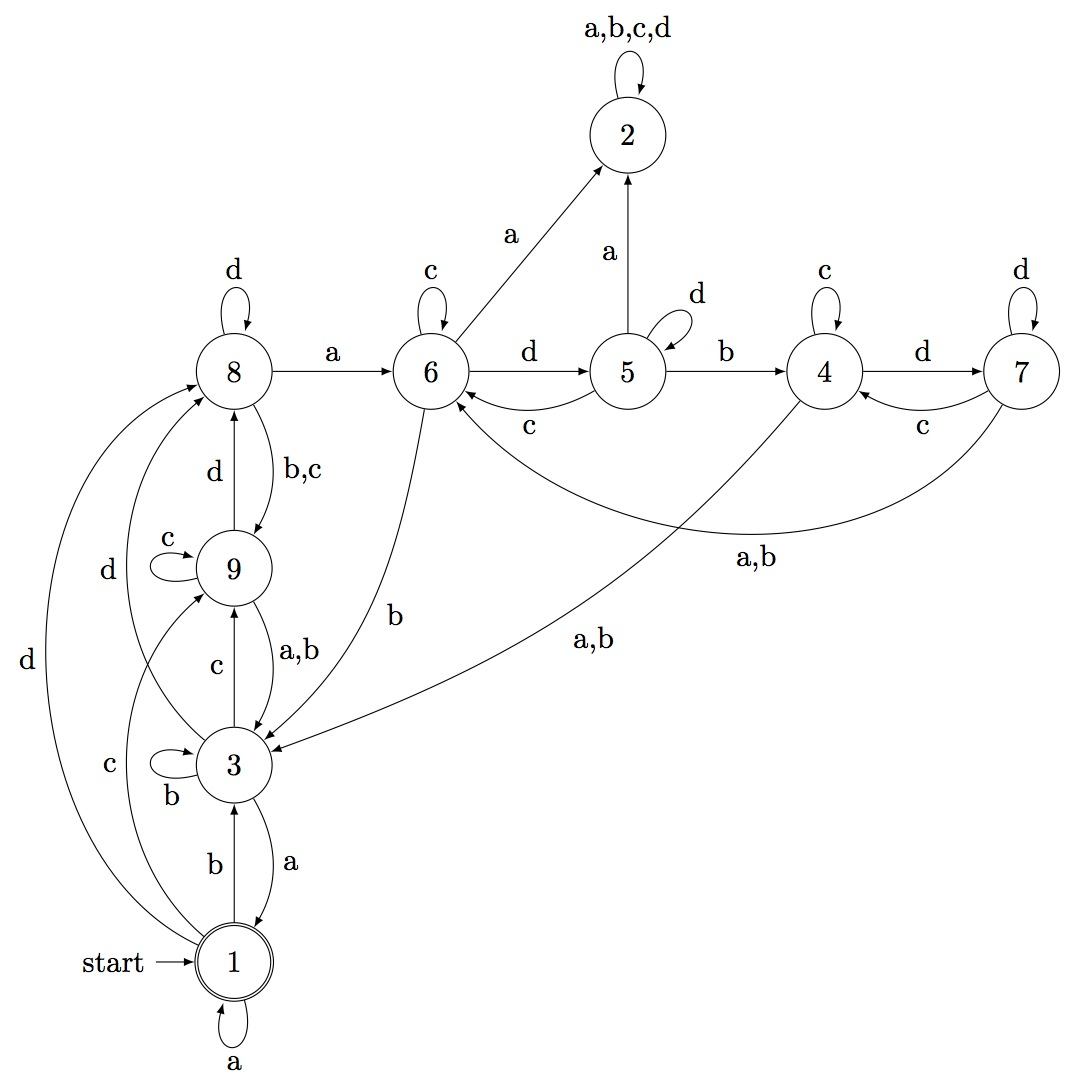
\includegraphics[scale=0.75]{img/ps22aut.jpg} \end{center}
\end{figure}   
\begin{Verbatim}[commandchars=!@C,fontsize=\small,frame=single,label=Example]
  !gapprompt@gap>C !gapinput@x:=BufferAndStack(3,2);C
  [ [ 2 .. 4 ], [ 5 ], [ 5 ], [ 5 ], [ 6, 7 ], [ 5 ], [  ] ]
  !gapprompt@gap>C !gapinput@aut:=GraphToAut(x,1,7);C
  < epsilon automaton on 5 letters with 460 states >
  !gapprompt@gap>C !gapinput@aut:=MinimalAutomaton(aut);C
  < deterministic automaton on 4 letters with 4 states >
  !gapprompt@gap>C !gapinput@Display(aut);C
     |  1  2  3  4  
  -----------------
   a |  1  4  1  3  
   b |  3  4  3  3  
   c |  4  4  4  4  
   d |  2  2  2  2  
  Initial state:   [ 1 ]
  Accepting state: [ 1 ]
  !gapprompt@gap>C !gapinput@C
\end{Verbatim}
  The following automaton represents the language of rank encoded permutations
that are output by \texttt{BufferAndStack(3,2)}: \begin{figure}[H] \begin{center} \leavevmode
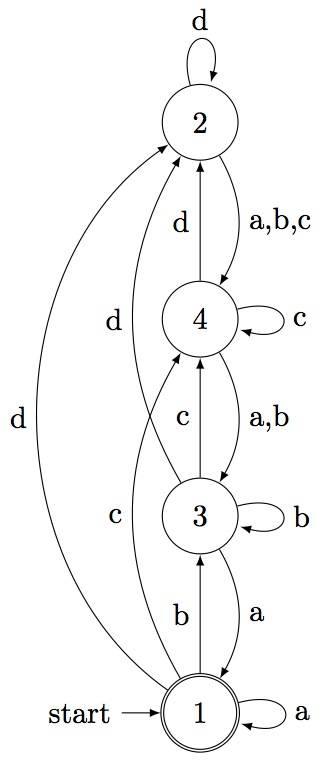
\includegraphics[scale=0.75]{img/bs32aut.jpg} \end{center} \end{figure}   
\begin{Verbatim}[commandchars=!@B,fontsize=\small,frame=single,label=Example]
  !gapprompt@gap>B !gapinput@x:=[[2,3],[4],[5],[3,6],[6],[]];B
  [ [ 2, 3 ], [ 4 ], [ 5 ], [ 3, 6 ], [ 6 ], [  ] ]
  !gapprompt@gap>B !gapinput@aut:=GraphToAut(x,1,6);B
  < epsilon automaton on 4 letters with 80 states >
  !gapprompt@gap>B !gapinput@aut:=MinimalAutomaton(aut);B
  < deterministic automaton on 3 letters with 8 states >
  !gapprompt@gap>B !gapinput@Display(aut);B
     |  1  2  3  4  5  6  7  8  
  -----------------------------
   a |  1  3  1  4  6  1  6  1  
   b |  3  8  3  4  4  6  6  6  
   c |  2  2  2  4  5  5  7  7  
  Initial state:   [ 1 ]
  Accepting state: [ 1 ]
  !gapprompt@gap>B !gapinput@B
\end{Verbatim}
 The input TPN here is the first network described in Chapter \ref{tpn}.  The language of rank encoded permutations of this token passing network is
accepted by the following automaton: \begin{figure}[H] \begin{center}
\leavevmode 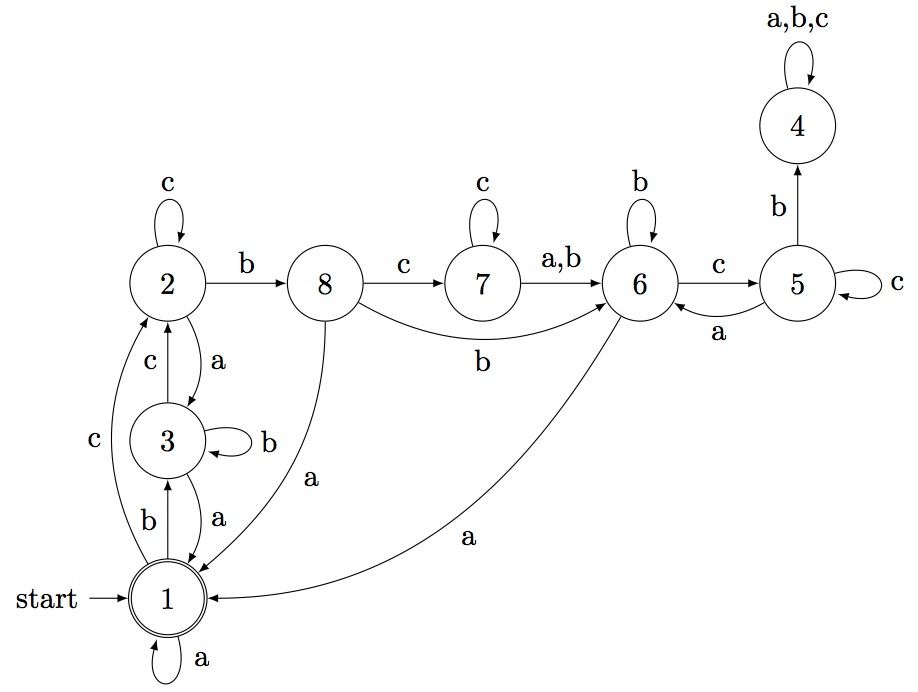
\includegraphics[scale=0.75]{img/hexaut.jpg} \end{center}
\end{figure}   }

 

\subsection{\textcolor{Chapter }{ConstrainedGraphToAut}}
\logpage{[ 4, 1, 2 ]}\nobreak
\hyperdef{L}{X7D457B517F2FDDA9}{}
{\noindent\textcolor{FuncColor}{$\triangleright$\ \ \texttt{ConstrainedGraphToAut({\mdseries\slshape g, innode, outnode, capacity})\index{ConstrainedGraphToAut@\texttt{ConstrainedGraphToAut}}
\label{ConstrainedGraphToAut}
}\hfill{\scriptsize (function)}}\\
\textbf{\indent Returns:\ }
An automaton representing the input TPN with bounded capacity.



 \texttt{ConstrainedGraphToAut} builds an epsilon automaton based on the same idea as \texttt{GraphToAut}, so it takes a list representation of a directed graph, a designated input
node and a distinct output node, but additionally there is the constraint that
there can be at most \texttt{capacity} tokens in the graph, at any time. 
\begin{Verbatim}[commandchars=!@B,fontsize=\small,frame=single,label=Example]
  !gapprompt@gap>B !gapinput@x:=Seqstacks(2,2);                  B
  [ [ 2 ], [ 3, 4 ], [ 2 ], [ 5, 6 ], [ 4 ], [  ] ]
  !gapprompt@gap>B !gapinput@aut:=ConstrainedGraphToAut(x,1,6,2);B
  < epsilon automaton on 6 letters with 21 states >
  !gapprompt@gap>B !gapinput@aut:=MinimalAutomaton(aut);         B
  < deterministic automaton on 5 letters with 3 states >
  !gapprompt@gap>B !gapinput@Display(aut);                       B
     |  1  2  3  
  --------------
   a |  1  2  1  
   b |  3  2  3  
   c |  2  2  2  
   d |  2  2  2  
   e |  2  2  2  
  Initial state:   [ 1 ]
  Accepting state: [ 1 ]
  !gapprompt@gap>B !gapinput@B
\end{Verbatim}
  The rank encoded permutations of \texttt{Seqstacks(2,2)}, where at any time there are at most 2 tokens within the network, are
accepted by the following automaton: \begin{figure}[H] \begin{center}
\leavevmode 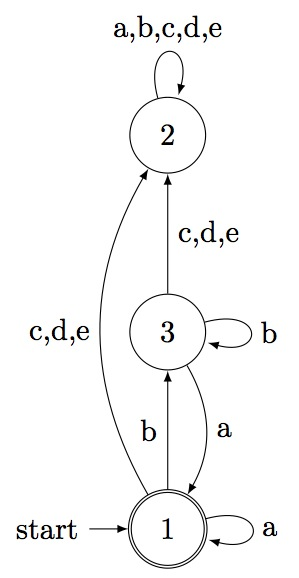
\includegraphics[scale=0.75]{img/ss22c2aut.jpg} \end{center}
\end{figure}   
\begin{Verbatim}[commandchars=!@E,fontsize=\small,frame=single,label=Example]
  !gapprompt@gap>E !gapinput@x:=BufferAndStack(3,2);      E
  [ [ 2 .. 4 ], [ 5 ], [ 5 ], [ 5 ], [ 6, 7 ], [ 5 ], [  ] ]
  !gapprompt@gap>E !gapinput@aut:=ConstrainedGraphToAut(x,1,6,3);E
  < epsilon automaton on 7 letters with 112 states >
  !gapprompt@gap>E !gapinput@aut:=MinimalAutomaton(aut);E
  < deterministic automaton on 6 letters with 4 states >
  !gapprompt@gap>E !gapinput@Display(aut);E
     |  1  2  3  4  
  -----------------
   a |  1  2  1  3  
   b |  3  2  3  3  
   c |  4  2  4  4  
   d |  2  2  2  2  
   e |  2  2  2  2  
   f |  2  2  2  2  
  Initial state:   [ 1 ]
  Accepting state: [ 1 ]
  !gapprompt@gap>E !gapinput@E
\end{Verbatim}
  The automaton corresponding to \texttt{BufferAndStack(3,2)} with limited capacity of 3 tokens is: \begin{figure}[H] \begin{center}
\leavevmode 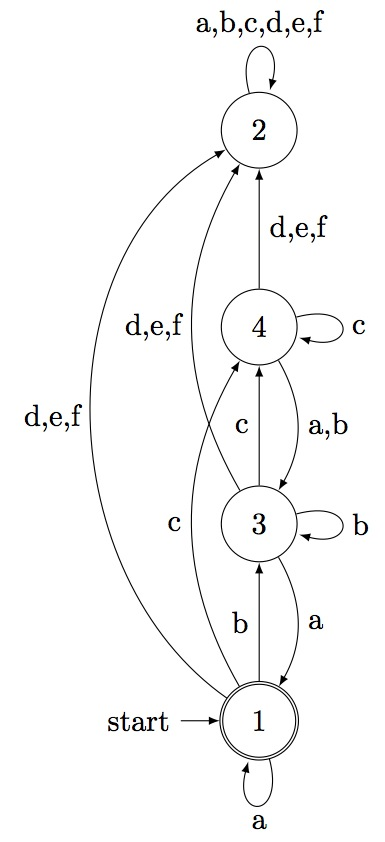
\includegraphics[scale=0.75]{img/bs32c3aut.jpg} \end{center}
\end{figure}   
\begin{Verbatim}[commandchars=!@B,fontsize=\small,frame=single,label=Example]
  !gapprompt@gap>B !gapinput@x:=[[2,3],[4],[5],[3,6],[6],[]];                      B
  [ [ 2, 3 ], [ 4 ], [ 5 ], [ 3, 6 ], [ 6 ], [  ] ]
  !gapprompt@gap>B !gapinput@aut:=ConstrainedGraphToAut(x,1,6,3);B
  < epsilon automaton on 6 letters with 48 states >
  !gapprompt@gap>B !gapinput@aut:=MinimalAutomaton(aut);         B
  < deterministic automaton on 5 letters with 8 states >
  !gapprompt@gap>B !gapinput@Display(aut);                       B
     |  1  2  3  4  5  6  7  8  
  -----------------------------
   a |  1  3  1  4  6  1  6  1  
   b |  3  8  3  4  4  6  6  6  
   c |  2  2  2  4  5  5  7  7  
   d |  4  4  4  4  4  4  4  4  
   e |  4  4  4  4  4  4  4  4  
  Initial state:   [ 1 ]
  Accepting state: [ 1 ]
  !gapprompt@gap>B !gapinput@B
\end{Verbatim}
  The automaton that accepts the language of rank encoded permutations of the
token passing network, from Chapter \ref{tpn}, with at most 3 tokens in the network at anytime, is: \begin{figure}[H]
\begin{center} \leavevmode 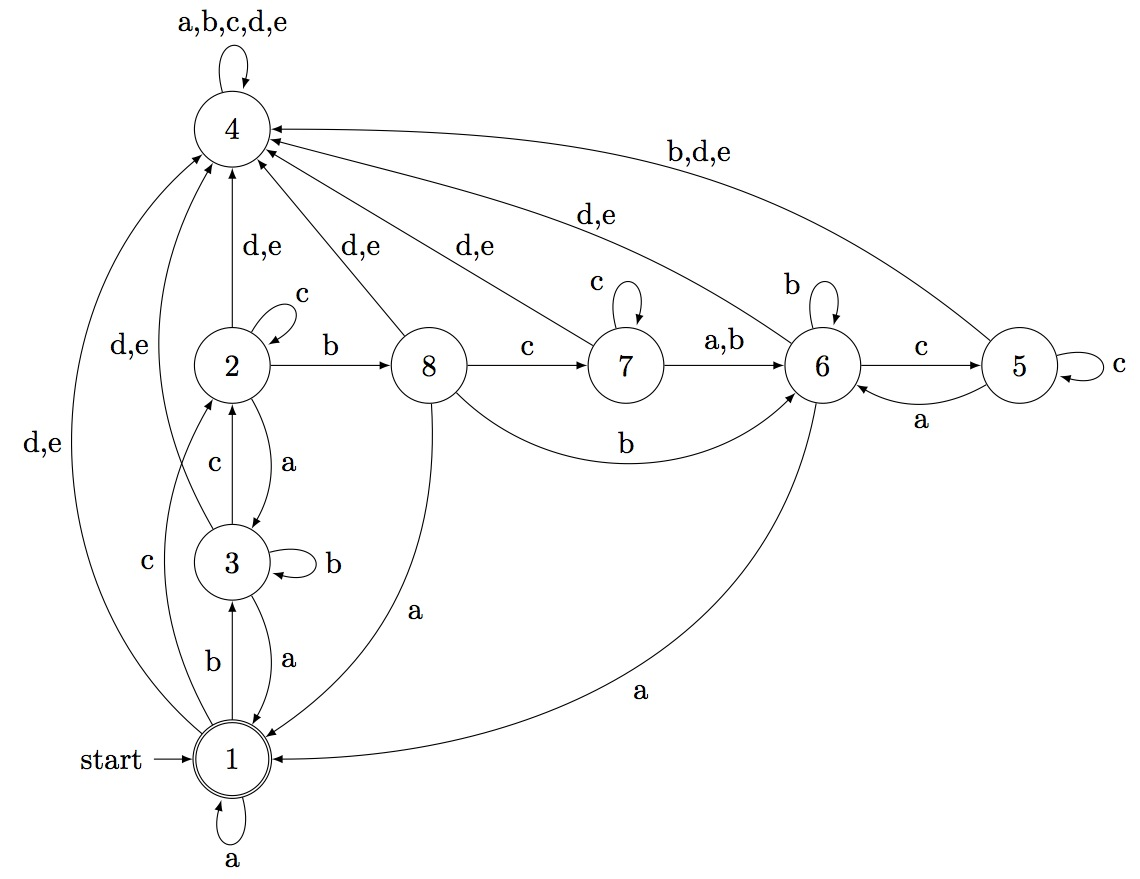
\includegraphics[scale=0.75]{img/hexc3aut.jpg}
\end{center} \end{figure}   }

 }

 }

 
\chapter{\textcolor{Chapter }{From Automata to Networks}}\logpage{[ 5, 0, 0 ]}
\hyperdef{L}{X78223796785BC628}{}
{
 It is not only important to see how a TPN can be interpreted as a finite state
automaton. But also if an arbitrary automaton could represent the language of
rank encoded permutations of a TPN. Currently within \texttt{PatternClass} it is only possible to check whether deterministic automata are possible
representatives of a TPN. 
\section{\textcolor{Chapter }{Functions}}\logpage{[ 5, 1, 0 ]}
\hyperdef{L}{X86FA580F8055B274}{}
{
 

\subsection{\textcolor{Chapter }{IsStarClosed}}
\logpage{[ 5, 1, 1 ]}\nobreak
\hyperdef{L}{X7E1DAEB979824B68}{}
{\noindent\textcolor{FuncColor}{$\triangleright$\ \ \texttt{IsStarClosed({\mdseries\slshape aut})\index{IsStarClosed@\texttt{IsStarClosed}}
\label{IsStarClosed}
}\hfill{\scriptsize (function)}}\\
\textbf{\indent Returns:\ }
 \texttt{true} if the start and accept states in \texttt{aut} are one and the same state. 



 This has the consequence that the whole rational expression accepted by \texttt{aut} is always enclosed by the Kleene star. 
\begin{Verbatim}[commandchars=!@|,fontsize=\small,frame=single,label=Example]
  !gapprompt@gap>| !gapinput@x:=Automaton("det",4,2,[[3,4,2,4],[2,2,2,4]],[1],[2]);|
  < deterministic automaton on 2 letters with 4 states >
  !gapprompt@gap>| !gapinput@IsStarClosed(x);                                      |
  false
  !gapprompt@gap>| !gapinput@AutToRatExp(x);        |
  (a(aUb)Ub)b*
  !gapprompt@gap>| !gapinput@y:=Automaton("det",3,2,[[3,2,1],[2,3,1]],[1],[1]);|
  < deterministic automaton on 2 letters with 3 states >
  !gapprompt@gap>| !gapinput@IsStarClosed(y);|
  true
  !gapprompt@gap>| !gapinput@AutToRatExp(y);|
  ((ba*bUa)(aUb))*
  !gapprompt@gap>| !gapinput@|
\end{Verbatim}
 }

 

\subsection{\textcolor{Chapter }{Is2StarReplaceable}}
\logpage{[ 5, 1, 2 ]}\nobreak
\hyperdef{L}{X873324D67DC9DC41}{}
{\noindent\textcolor{FuncColor}{$\triangleright$\ \ \texttt{Is2StarReplaceable({\mdseries\slshape aut})\index{Is2StarReplaceable@\texttt{Is2StarReplaceable}}
\label{Is2StarReplaceable}
}\hfill{\scriptsize (function)}}\\
\textbf{\indent Returns:\ }
 \texttt{true} if none of the states in the automaton \texttt{aut}, which are not the initial state, have a transition to the initial state
labelled with the first letter of the alphabet. It also returns \texttt{true} if there is at least one state $i \in Q$ with the first two transitions from $i$ being $f(i,1)=1$ and $f(i,2)=x$, where $x \in Q\setminus\{1\}$ and $f(x,1)=1$.



 
\begin{Verbatim}[commandchars=!@|,fontsize=\small,frame=single,label=Example]
  !gapprompt@gap>| !gapinput@x:=Automaton("det",3,2,[[1,2,3],[2,2,3]],[1],[2]);|
  < deterministic automaton on 2 letters with 3 states >
  !gapprompt@gap>| !gapinput@Is2StarReplaceable(x);|
  true
  !gapprompt@gap>| !gapinput@y:=Automaton("det",4,2,[[4,1,1,2],[1,3,3,2]],[1],[1]);|
  < deterministic automaton on 2 letters with 4 states >
  !gapprompt@gap>| !gapinput@Is2StarReplaceable(y);|
  true
  !gapprompt@gap>| !gapinput@z:=Automaton("det",4,2,[[4,1,1,2],[1,4,2,2]],[1],[4]);|
  < deterministic automaton on 2 letters with 4 states >
  !gapprompt@gap>| !gapinput@Is2StarReplaceable(z);|
  false
  !gapprompt@gap>| !gapinput@|
\end{Verbatim}
 }

 

\subsection{\textcolor{Chapter }{IsStratified}}
\logpage{[ 5, 1, 3 ]}\nobreak
\hyperdef{L}{X7FF528F784C9020B}{}
{\noindent\textcolor{FuncColor}{$\triangleright$\ \ \texttt{IsStratified({\mdseries\slshape aut})\index{IsStratified@\texttt{IsStratified}}
\label{IsStratified}
}\hfill{\scriptsize (function)}}\\
\textbf{\indent Returns:\ }
\texttt{true} if \texttt{aut} has a specific "layered" form.



 A formal description of the most basic stratified automaton is: 

 $(S,Q,f,q_{0},A)$ with $S:=\{1,...,n\},\,\, Q:=\{1,...,m\},\,\, n<m,\,\, q_{0}:=1,\,\, A:=Q\setminus
\{n+1\},\,\, f: Q \times S \rightarrow Q $ and $n+1$ is a sink state. 

 If $i,j \in Q \setminus \{ n+1 \}$,with $i < j$, and $i',j' \in S$, $i=i',\,\, j=j'$ then 
\[f(i,i')=i,\,\, f(i,j')=j,\,\, f(j,j')=j,\,\, f(j,i')=j-1 \,\, or \,\, n+1.\]
 
\begin{Verbatim}[commandchars=!@|,fontsize=\small,frame=single,label=Example]
  !gapprompt@gap>| !gapinput@x:=Automaton("det",4,2,[[1,3,1,4],[2,2,4,4]],[1],[2]);|
  < deterministic automaton on 2 letters with 4 states >
  !gapprompt@gap>| !gapinput@IsStratified(x);                                      |
  true
  !gapprompt@gap>| !gapinput@y:=Automaton("det",4,2,[[1,3,2,4],[2,4,1,4]],[1],[2]);|
  < deterministic automaton on 2 letters with 4 states >
  !gapprompt@gap>| !gapinput@IsStratified(y);                                      |
  false
  !gapprompt@gap>| !gapinput@|
\end{Verbatim}
 }

 

\subsection{\textcolor{Chapter }{IsPossibleGraphAut}}
\logpage{[ 5, 1, 4 ]}\nobreak
\hyperdef{L}{X7C3B9EB080F72043}{}
{\noindent\textcolor{FuncColor}{$\triangleright$\ \ \texttt{IsPossibleGraphAut({\mdseries\slshape aut})\index{IsPossibleGraphAut@\texttt{IsPossibleGraphAut}}
\label{IsPossibleGraphAut}
}\hfill{\scriptsize (function)}}\\
\textbf{\indent Returns:\ }
 \texttt{true} if \texttt{aut} returns \texttt{true} in \texttt{IsStratified}, \texttt{Is2StarReplaceable} and \texttt{IsStarClosed}.



 An automaton that fulfils the three functions above has the right form to be
an automaton representing rank encoded permutations, which are output from a
TPN. 
\begin{Verbatim}[commandchars=!@|,fontsize=\small,frame=single,label=Example]
  !gapprompt@gap>| !gapinput@x:=Automaton("det",2,2,[[1,2],[2,2]],[1],[1]);|
  < deterministic automaton on 2 letters with 2 states >
  !gapprompt@gap>| !gapinput@IsPossibleGraphAut(x);|
  true
  !gapprompt@gap>| !gapinput@y:=Automaton("det",2,2,[[1,2],[1,2]],[1],[1]);|
  < deterministic automaton on 2 letters with 2 states >
  !gapprompt@gap>| !gapinput@IsPossibleGraphAut(y);                        |
  false
  !gapprompt@gap>| !gapinput@IsStarClosed(y);|
  true
  !gapprompt@gap>| !gapinput@Is2StarReplaceable(y);|
  true
  !gapprompt@gap>| !gapinput@IsStratified(y);|
  false
  !gapprompt@gap>| !gapinput@|
\end{Verbatim}
 }

 }

 }

 
\chapter{\textcolor{Chapter }{Pattern Classes}}\logpage{[ 6, 0, 0 ]}
\hyperdef{L}{X85A198CB7EBA4BDE}{}
{
 Permutation pattern classes can be determined using their corresponding basis.
The basis of a pattern class is the anti-chain of the class, under the order
of containment. A permutation $\pi$ contains another permutation $\sigma$ (of shorter length) if there is a subsequence in $\pi$, which is isomorphic to $\sigma$. 

 With the rational language of the rank encoded class, it is also possible to
find the rational language of the basis and vice versa. Several specific kinds
of transducers are used in this process. \cite{RegCloSetPerms} 
\section{\textcolor{Chapter }{Transducers}}\logpage{[ 6, 1, 0 ]}
\hyperdef{L}{X843CB33182B8E477}{}
{
 

\subsection{\textcolor{Chapter }{Transducer}}
\logpage{[ 6, 1, 1 ]}\nobreak
\hyperdef{L}{X7A2DA7017E4F6BC4}{}
{\noindent\textcolor{FuncColor}{$\triangleright$\ \ \texttt{Transducer({\mdseries\slshape states, init, transitions, accepting})\index{Transducer@\texttt{Transducer}}
\label{Transducer}
}\hfill{\scriptsize (function)}}\\
\textbf{\indent Returns:\ }
A record that represents a transducer.



 A transducer is essentially an automaton, where running through the process
does not determine whether the input is accepted, but the input is translated
to another language, over a different alphabet. 

 Formally a transducer is a six-tuple with: $Q$ being the set of states, $S$ the input alphabet, $G$ the output alphabet, $I \in Q$ the start state, $A \subseteq Q$ the set of accept states, and with the transition function $f: Q \times (S \cup \{e\}) \rightarrow Q \times (G \cup \{e\})$, where $e$ is the empty word. 

 In this function the transducer is stored by defining how many states there
are, which one (by index) is the start or initial state, the transitions are
of the form \texttt{[inputletter,outputletter,fromstate,tostate]} and a list of accept states. The input and output alphabet are determined by
the input and output letters on the transitions. 
\begin{Verbatim}[commandchars=!@|,fontsize=\small,frame=single,label=Example]
  !gapprompt@gap>| !gapinput@trans:=Transducer(3,1,[[1,2,1,2],[1,2,2,2],[2,2,1,3],[2,2,2,3],|
  !gapprompt@>| !gapinput@[1,1,3,3],[2,2,3,3]],[2]);|
  rec( accepting := [ 2 ], initial := 1, states := 3, 
    transitions := [ [ 1, 2, 1, 2 ], [ 1, 2, 2, 2 ], [ 2, 2, 1, 3 ], 
        [ 2, 2, 2, 3 ], [ 1, 1, 3, 3 ], [ 2, 2, 3, 3 ] ] )
  !gapprompt@gap>| !gapinput@|
\end{Verbatim}
  This transducer can be visualised as the following graph: \begin{figure}[H]
\begin{center} \leavevmode 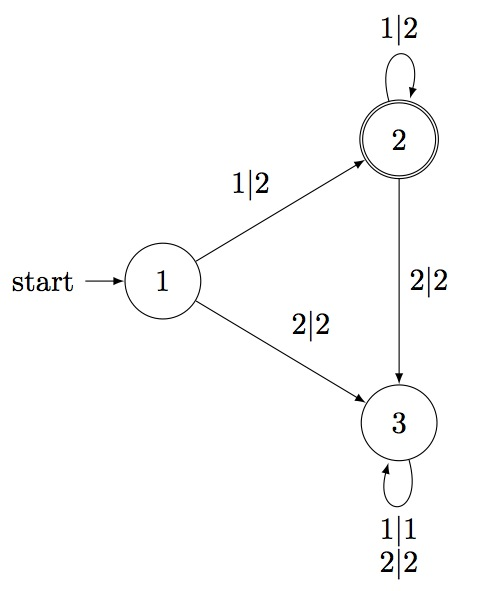
\includegraphics[scale=0.75]{img/trans.jpg}
\end{center} \end{figure}   }

 

\subsection{\textcolor{Chapter }{DeletionTransducer}}
\logpage{[ 6, 1, 2 ]}\nobreak
\hyperdef{L}{X7EB2EA8C78DA1F74}{}
{\noindent\textcolor{FuncColor}{$\triangleright$\ \ \texttt{DeletionTransducer({\mdseries\slshape k})\index{DeletionTransducer@\texttt{DeletionTransducer}}
\label{DeletionTransducer}
}\hfill{\scriptsize (function)}}\\
\textbf{\indent Returns:\ }
A transducer over \texttt{k}+1 states.



 A deletion transducer is a transducer that deletes one letter of a rank
encoded permutation and returns the correct rank encoding of the new
permutation. The deletion transducer over \texttt{k} deletes letters over the set of all rank encoded permutations with highest
rank \texttt{k}. Specifically, running through a deletion transducer with a rank encoded
permutation, of highest rank \texttt{k}, will lead to the set of all rank encoded permutations that have one letter
of the initial permutation removed. It is important to note that computing
these shorter permutations with the transducer, is done by reading the input
permutation from right to left. For example the deletion transducer with \texttt{k}=3, looks as follows: 
\begin{Verbatim}[commandchars=!@|,fontsize=\small,frame=single,label=Example]
  !gapprompt@gap>| !gapinput@DeletionTransducer(3);|
  rec( accepting := [ 1 .. 3 ], initial := 4, states := 4, 
    transitions := [ [ 1, 1, 4, 4 ], [ 1, 0, 4, 1 ], [ 2, 1, 1, 1 ], 
        [ 1, 1, 1, 2 ], [ 3, 2, 1, 1 ], [ 1, 1, 2, 3 ], [ 1, 1, 3, 3 ], 
        [ 2, 2, 4, 4 ], [ 2, 0, 4, 2 ], [ 3, 2, 2, 2 ], [ 2, 2, 2, 3 ], 
        [ 2, 2, 3, 3 ], [ 3, 3, 4, 4 ], [ 3, 0, 4, 3 ], [ 3, 3, 3, 3 ] ] )
  !gapprompt@gap>| !gapinput@|
\end{Verbatim}
  \begin{figure}[H] \begin{center} \leavevmode
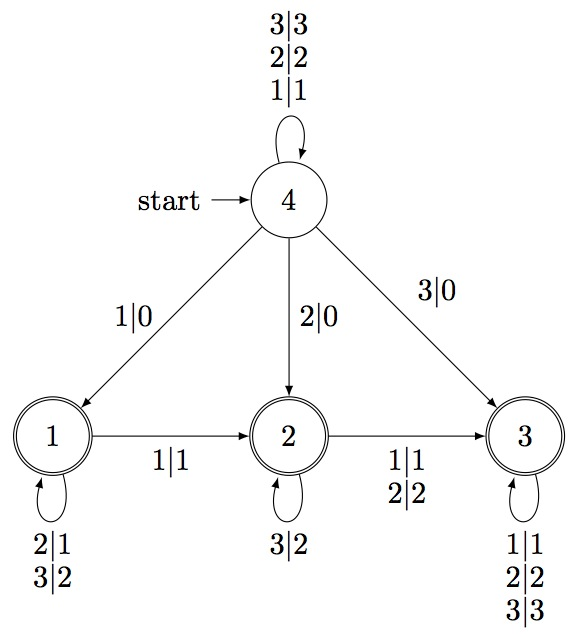
\includegraphics[scale=0.75]{img/dt3.jpg} \end{center} \end{figure}   }

 

\subsection{\textcolor{Chapter }{TransposedTransducer}}
\logpage{[ 6, 1, 3 ]}\nobreak
\hyperdef{L}{X85711F837F30E225}{}
{\noindent\textcolor{FuncColor}{$\triangleright$\ \ \texttt{TransposedTransducer({\mdseries\slshape t})\index{TransposedTransducer@\texttt{TransposedTransducer}}
\label{TransposedTransducer}
}\hfill{\scriptsize (function)}}\\
\textbf{\indent Returns:\ }
A new transducer with interchanged input and output letters on each
transition.



 A transducer is transposed when all origins and destinations of transitions
are left the same as before but the input and output letters on each
transition are interchanged. Taking the deletion transducer from above, its
transpose looks as follows: 
\begin{Verbatim}[commandchars=!@|,fontsize=\small,frame=single,label=Example]
  !gapprompt@gap>| !gapinput@TransposedTransducer(DeletionTransducer(3));|
  rec( accepting := [ 1 .. 3 ], initial := 4, states := 4, 
    transitions := [ [ 1, 1, 4, 4 ], [ 0, 1, 4, 1 ], [ 1, 2, 1, 1 ], 
        [ 1, 1, 1, 2 ], [ 2, 3, 1, 1 ], [ 1, 1, 2, 3 ], [ 1, 1, 3, 3 ], 
        [ 2, 2, 4, 4 ], [ 0, 2, 4, 2 ], [ 2, 3, 2, 2 ], [ 2, 2, 2, 3 ], 
        [ 2, 2, 3, 3 ], [ 3, 3, 4, 4 ], [ 0, 3, 4, 3 ], [ 3, 3, 3, 3 ] ] )
  !gapprompt@gap>| !gapinput@|
\end{Verbatim}
  \begin{figure}[H] \begin{center} \leavevmode
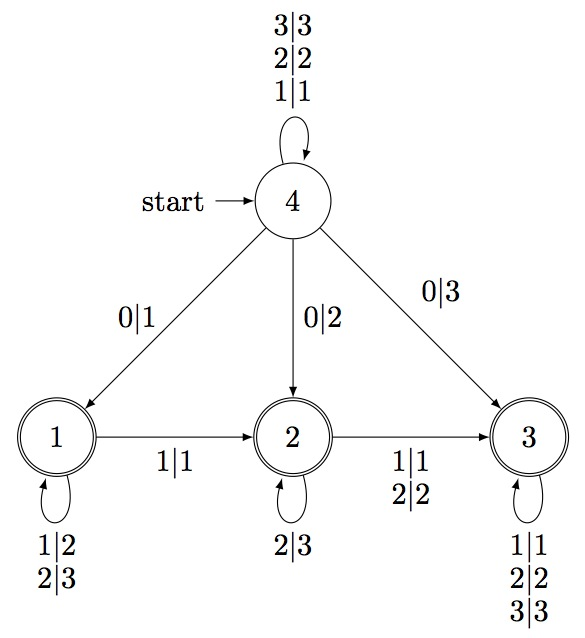
\includegraphics[scale=0.75]{img/dtt3.jpg} \end{center} \end{figure}   }

 

\subsection{\textcolor{Chapter }{InvolvementTransducer}}
\logpage{[ 6, 1, 4 ]}\nobreak
\hyperdef{L}{X7BBBA46E84BDD089}{}
{\noindent\textcolor{FuncColor}{$\triangleright$\ \ \texttt{InvolvementTransducer({\mdseries\slshape k})\index{InvolvementTransducer@\texttt{InvolvementTransducer}}
\label{InvolvementTransducer}
}\hfill{\scriptsize (function)}}\\
\textbf{\indent Returns:\ }
A transducer over \texttt{k}+1 states, with a \texttt{k} sized alphabet.



 An involvement transducer is a transducer over \texttt{k}+1 states, and deletes any number of letters in a rank encoded permutation, of
rank at most \texttt{k}. 
\begin{Verbatim}[commandchars=!@|,fontsize=\small,frame=single,label=Example]
  !gapprompt@gap>| !gapinput@InvolvementTransducer(3);|
  rec( accepting := [ 1 .. 4 ], initial := 4, states := 4, 
    transitions := [ [ 1, 1, 1, 2 ], [ 1, 0, 1, 3 ], [ 2, 1, 1, 1 ], 
        [ 2, 0, 1, 3 ], [ 3, 2, 1, 1 ], [ 3, 0, 1, 1 ], [ 1, 1, 2, 4 ], 
        [ 1, 0, 2, 1 ], [ 2, 2, 2, 4 ], [ 2, 0, 2, 2 ], [ 3, 2, 2, 2 ], 
        [ 3, 0, 2, 2 ], [ 1, 1, 3, 2 ], [ 1, 0, 3, 3 ], [ 2, 1, 3, 1 ], 
        [ 2, 0, 3, 3 ], [ 3, 1, 3, 3 ], [ 3, 0, 3, 3 ], [ 1, 1, 4, 4 ], 
        [ 1, 0, 4, 1 ], [ 2, 2, 4, 4 ], [ 2, 0, 4, 2 ], [ 3, 3, 4, 4 ], 
        [ 3, 0, 4, 4 ] ] )
  !gapprompt@gap>| !gapinput@|
\end{Verbatim}
  \begin{figure}[H] \begin{center} \leavevmode
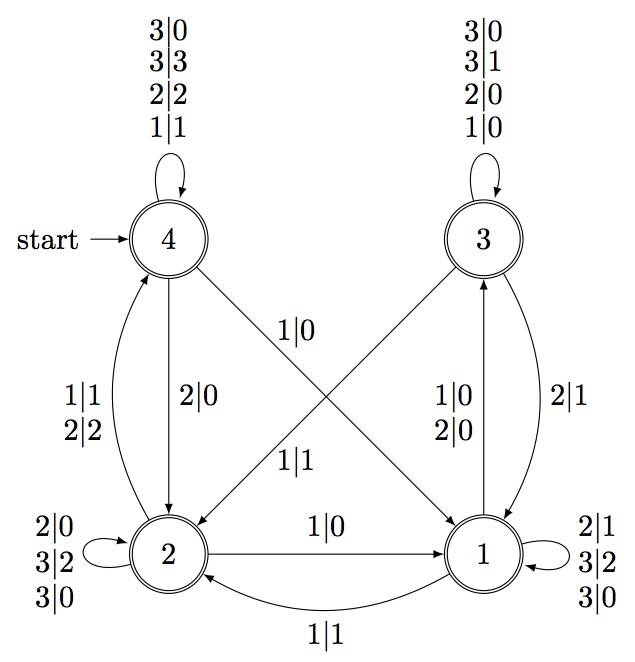
\includegraphics[scale=0.75]{img/it3.jpg} \end{center} \end{figure}   }

 

\subsection{\textcolor{Chapter }{CombineAutTransducer}}
\logpage{[ 6, 1, 5 ]}\nobreak
\hyperdef{L}{X7E41CAC57CE71CB1}{}
{\noindent\textcolor{FuncColor}{$\triangleright$\ \ \texttt{CombineAutTransducer({\mdseries\slshape aut, trans})\index{CombineAutTransducer@\texttt{CombineAutTransducer}}
\label{CombineAutTransducer}
}\hfill{\scriptsize (function)}}\\
\textbf{\indent Returns:\ }
An automaton consisting of a combination of \texttt{aut} and \texttt{trans}.



 Combining automata and transducers is done over the natural "translation" of
the by the automaton accepted language through the transducer and then
building a new automaton that accepts the new language. The function \texttt{CombineAutTransducer} does this process and returns the new non-deterministic automaton. 
\begin{Verbatim}[commandchars=!@B,fontsize=\small,frame=single,label=Example]
  !gapprompt@gap>B !gapinput@a:=Automaton("det",1,1,[[1]],[1],[1]);B
  < deterministic automaton on 1 letters with 1 states >
  !gapprompt@gap>B !gapinput@AutToRatExp(a);B
  a*
  !gapprompt@gap>B !gapinput@t:=Transducer(2,1,[[1,2,1,2],[2,1,1,2],B
  !gapprompt@>B !gapinput@[1,1,2,1],[2,2,2,1]],[1]);B
  rec( accepting := [ 1 ], initial := 1, states := 2, 
    transitions := [ [ 1, 2, 1, 2 ], [ 2, 1, 1, 2 ], [ 1, 1, 2, 1 ], 
        [ 2, 2, 2, 1 ] ] )
  !gapprompt@gap>B !gapinput@res:=CombineAutTransducer(a,t);B
  < non deterministic automaton on 2 letters with 2 states >
  !gapprompt@gap>B !gapinput@AutToRatExp(res);B
  (ba)*
  !gapprompt@gap>B !gapinput@Display(res);B
     |  1       2
  -------------------
   a |         [ 1 ]   
   b | [ 2 ]           
  Initial state:   [ 1 ]
  Accepting state: [ 1 ]
  !gapprompt@gap>B !gapinput@B
\end{Verbatim}
 }

 }

 
\section{\textcolor{Chapter }{From Class to Basis and vice versa}}\logpage{[ 6, 2, 0 ]}
\hyperdef{L}{X7CFEC6DB7CA880CC}{}
{
 

\subsection{\textcolor{Chapter }{BasisAutomaton}}
\logpage{[ 6, 2, 1 ]}\nobreak
\hyperdef{L}{X7FD8B2357CAAFC0B}{}
{\noindent\textcolor{FuncColor}{$\triangleright$\ \ \texttt{BasisAutomaton({\mdseries\slshape a})\index{BasisAutomaton@\texttt{BasisAutomaton}}
\label{BasisAutomaton}
}\hfill{\scriptsize (function)}}\\
\textbf{\indent Returns:\ }
An automaton that accepts the rank encoded permutations of the basis of the
input automaton \texttt{a}.



 Every pattern class has a basis that consists of the smallest set of
permutations which do not belong to the class. Using 
\[B(L)=(L^{r} D^{t})^{r} \cap L^{c}\]
 it is possible using the deletion transducer $D$ and the language of rank encoded permutations $L$ to find the language of the rank encoded permutations of the basis $B(L)$, and thus the basis. 
\begin{Verbatim}[commandchars=!CF,fontsize=\small,frame=single,label=Example]
  !gappromptCgap>F !gapinputCx:=Parstacks(2,2);F
  [ [ 2, 4 ], [ 3, 6 ], [ 2 ], [ 5, 6 ], [ 4 ], [  ] ]
  !gappromptCgap>F !gapinputCxa:=GraphToAut(x,1,6);F
  < epsilon automaton on 5 letters with 66 states >
  !gappromptCgap>F !gapinputCma:=MinimalAutomaton(xa);F
  < deterministic automaton on 4 letters with 9 states >
  !gappromptCgap>F !gapinputCDisplay(ma);F
     |  1  2  3  4  5  6  7  8  9  
  --------------------------------
   a |  1  2  1  3  2  2  6  6  3  
   b |  3  2  3  3  4  3  6  9  3  
   c |  9  2  9  4  6  6  4  9  9  
   d |  8  2  8  7  5  5  7  8  8  
  Initial state:   [ 1 ]
  Accepting state: [ 1 ]
  !gappromptCgap>F !gapinputCba:=BasisAutomaton(ma);F
  < deterministic automaton on 4 letters with 9 states >
  !gappromptCgap>F !gapinputCDisplay(ba);F
     |  1  2  3  4  5  6  7  8  9  
  --------------------------------
   a |  2  2  1  3  4  2  2  2  2  
   b |  2  2  2  2  2  4  1  2  8  
   c |  2  2  2  2  2  2  1  2  2  
   d |  2  2  2  9  2  2  5  6  2  
  Initial state:    [ 7 ]
  Accepting states: [ 1, 5 ]
  !gappromptCgap>F !gapinputCAutToRatExp(ba);F
  d(a(dbdb)*aaU@)UbUc
  !gappromptCgap>F !gapinputCF
\end{Verbatim}
 Ignoring the trailing \texttt{UbUc} which essentially are noise, the basis of the pattern class indicates which
permutations are avoided in this particular class. The shortest permutation in
the basis, looking at the rational expression, is $daaa$, which can be translated to 4111 and decoded to the permutation 4123. }

 

\subsection{\textcolor{Chapter }{ClassAutomaton}}
\logpage{[ 6, 2, 2 ]}\nobreak
\hyperdef{L}{X78BD24D7828004E8}{}
{\noindent\textcolor{FuncColor}{$\triangleright$\ \ \texttt{ClassAutomaton({\mdseries\slshape a})\index{ClassAutomaton@\texttt{ClassAutomaton}}
\label{ClassAutomaton}
}\hfill{\scriptsize (function)}}\\
\textbf{\indent Returns:\ }
The automaton that accepts permutations of the class in their rank encoding.



 The function \texttt{ClassAutomaton} does the reverse process of \texttt{BasisAutomaton}. Namely it takes the automaton that represents the language of the rank
encoded basis of a permutation class, and using the formula 
\[L=B_{k} \cap ((B(L)^{r} I^{t})^{c} )^{r}\]
 returns the automaton that accepts the rank encoded permutations of the class.
In the formula, $B_{k}$ is the automaton that accepts all permutations of any length with highest rank $k$, $B(L)$ is the automaton that represents the basis and $I$ is the involement transducer. 
\begin{Verbatim}[commandchars=!@B,fontsize=\small,frame=single,label=Example]
  !gapprompt@gap>B !gapinput@xa:=Automaton("det",9,4,[[2,2,1,3,4,2,2,2,2],[2,2,2,2,2,4,1,2,8],B
  !gapprompt@>B !gapinput@[2,2,2,2,2,2,1,2,2],[2,2,2,9,2,2,5,6,2]],[7],[1,5]); B
  < deterministic automaton on 4 letters with 9 states >
  !gapprompt@gap>B !gapinput@ca:=ClassAutomaton(xa); B
  < deterministic automaton on 4 letters with 9 states >
  !gapprompt@gap>B !gapinput@Display(ca);B
     |  1  2  3  4  5  6  7  8  9  
  --------------------------------
   a |  1  2  1  3  2  2  6  6  3  
   b |  3  2  3  3  4  3  6  9  3  
   c |  9  2  9  4  6  6  4  9  9  
   d |  8  2  8  7  5  5  7  8  8  
  Initial state:   [ 1 ]
  Accepting state: [ 1 ]
  !gapprompt@gap>B !gapinput@IsPossibleGraphAut(ca);B
  true
  !gapprompt@gap>B !gapinput@B
\end{Verbatim}
 }

 

\subsection{\textcolor{Chapter }{BoundedClassAutomaton}}
\logpage{[ 6, 2, 3 ]}\nobreak
\hyperdef{L}{X856A6F5085BAA7C3}{}
{\noindent\textcolor{FuncColor}{$\triangleright$\ \ \texttt{BoundedClassAutomaton({\mdseries\slshape k})\index{BoundedClassAutomaton@\texttt{BoundedClassAutomaton}}
\label{BoundedClassAutomaton}
}\hfill{\scriptsize (function)}}\\
\textbf{\indent Returns:\ }
An automaton that accepts all rank encoded permutations, with highest rank
being \texttt{k}.



 The bounded class automaton, is an automaton that accepts all rank encoded
permutations, of any length, with highest rank \texttt{k}. 
\begin{Verbatim}[commandchars=!@E,fontsize=\small,frame=single,label=Example]
  !gapprompt@gap>E !gapinput@BoundedClassAutomaton(3);E
  < deterministic automaton on 3 letters with 3 states >
  !gapprompt@gap>E !gapinput@Display(last);E
     |  1  2  3  
  --------------
   a |  1  1  2  
   b |  2  2  2  
   c |  3  3  3  
  Initial state:   [ 1 ]
  Accepting state: [ 1 ]
  !gapprompt@gap>E !gapinput@E
\end{Verbatim}
 }

 

\subsection{\textcolor{Chapter }{ClassAutFromBaseEncoding}}
\logpage{[ 6, 2, 4 ]}\nobreak
\hyperdef{L}{X82D67FC587793580}{}
{\noindent\textcolor{FuncColor}{$\triangleright$\ \ \texttt{ClassAutFromBaseEncoding({\mdseries\slshape base, k})\index{ClassAutFromBaseEncoding@\texttt{ClassAutFromBaseEncoding}}
\label{ClassAutFromBaseEncoding}
}\hfill{\scriptsize (function)}}\\
\textbf{\indent Returns:\ }
The class automaton from a list of rank encoded basis permutations.



 Given the permutations in the basis, in their rank encoded form, and the bound
of the rank of the permutations of the class, \texttt{ClassAutFromBaseEncoding} builds the automaton that accepts rank encoded permutations of the class. 
\begin{Verbatim}[commandchars=!@G,fontsize=\small,frame=single,label=Example]
  !gapprompt@gap>G !gapinput@ClassAutFromBaseEncoding([[4,1,1,1]],4); G
  < deterministic automaton on 4 letters with 7 states >
  !gapprompt@gap>G !gapinput@Display(last);G
     |  1  2  3  4  5  6  7  
  --------------------------
   a |  1  2  1  3  2  2  6  
   b |  3  2  3  3  4  3  4  
   c |  4  2  4  4  6  6  4  
   d |  7  2  7  7  5  5  7  
  Initial state:   [ 1 ]
  Accepting state: [ 1 ]
  !gapprompt@gap>G !gapinput@G
\end{Verbatim}
 }

 

\subsection{\textcolor{Chapter }{ClassAutFromBase}}
\logpage{[ 6, 2, 5 ]}\nobreak
\hyperdef{L}{X80CBBEE08239B1B1}{}
{\noindent\textcolor{FuncColor}{$\triangleright$\ \ \texttt{ClassAutFromBase({\mdseries\slshape perms, k})\index{ClassAutFromBase@\texttt{ClassAutFromBase}}
\label{ClassAutFromBase}
}\hfill{\scriptsize (function)}}\\
\textbf{\indent Returns:\ }
The class automaton from a list of permutations of the basis.



 Taking \texttt{perms} which is the list of permutations in the basis and \texttt{k} an integer which indicates the highest rank in the encoded permutations of the
class, \texttt{ClassAutFromBase} constructs the automaton that accepts the language of rank encoded
permutations of the class.  
\begin{Verbatim}[commandchars=!@E,fontsize=\small,frame=single,label=Example]
  !gapprompt@gap>E !gapinput@ClassAutFromBase([[4,1,2,3]],4);E
  < deterministic automaton on 4 letters with 7 states >
  !gapprompt@gap>E !gapinput@Display(last);E
     |  1  2  3  4  5  6  7  
  --------------------------
   a |  1  2  1  3  2  2  6  
   b |  3  2  3  3  4  3  4  
   c |  4  2  4  4  6  6  4  
   d |  7  2  7  7  5  5  7  
  Initial state:   [ 1 ]
  Accepting state: [ 1 ]
  !gapprompt@gap>E !gapinput@E
\end{Verbatim}
 }

 

\subsection{\textcolor{Chapter }{ExpandAlphabet}}
\logpage{[ 6, 2, 6 ]}\nobreak
\hyperdef{L}{X877C8457804E4B45}{}
{\noindent\textcolor{FuncColor}{$\triangleright$\ \ \texttt{ExpandAlphabet({\mdseries\slshape a, newAlphabet})\index{ExpandAlphabet@\texttt{ExpandAlphabet}}
\label{ExpandAlphabet}
}\hfill{\scriptsize (function)}}\\
\textbf{\indent Returns:\ }
The automaton \texttt{a}, over the alphabet of size \texttt{newAlphabet}.



 Given an automaton and the size of the new alphabet, which has to be bigger
than the size of the alphabet in \texttt{a} , \texttt{ExpandAlphabet} changes the automaton \texttt{a} to contain an alphabet of size \texttt{newAlphabet}. The new letters have no transitions within the automaton. 
\begin{Verbatim}[commandchars=!@B,fontsize=\small,frame=single,label=Example]
  !gapprompt@gap>B !gapinput@aut:=Automaton("det",3,2,[[2,2,3],[3,3,3]],[1],[3]);B
  < deterministic automaton on 2 letters with 3 states >
  !gapprompt@gap>B !gapinput@Display(aut);B
     |  1  2  3  
  --------------
   a |  2  2  3  
   b |  3  3  3  
  Initial state:   [ 1 ]
  Accepting state: [ 3 ]
  !gapprompt@gap>B !gapinput@ExpandAlphabet(aut,4);B
  < deterministic automaton on 4 letters with 3 states >
  !gapprompt@gap>B !gapinput@Display(last);B
     |  1  2  3  
  --------------
   a |  2  2  3  
   b |  3  3  3  
   c |           
   d |           
  Initial state:   [ 1 ]
  Accepting state: [ 3 ]
  !gapprompt@gap>B !gapinput@B
\end{Verbatim}
 }

 }

 
\section{\textcolor{Chapter }{Direct Sum of Regular Classes}}\logpage{[ 6, 3, 0 ]}
\hyperdef{L}{X8218BF7787571EE0}{}
{
 It is obvious that the direct sum of two rational pattern classes is also
rational. But the skew sum of two rational pattern classes does not imply that
the resulting pattern class is rational, because if the second class in the
sum has infinitely many permutations, the alphabet of the skew sum class will
be infinite and thusly the resulting class will not be rational. 

\subsection{\textcolor{Chapter }{ClassDirectSum}}
\logpage{[ 6, 3, 1 ]}\nobreak
\hyperdef{L}{X7DC869E27CC3BFE0}{}
{\noindent\textcolor{FuncColor}{$\triangleright$\ \ \texttt{ClassDirectSum({\mdseries\slshape aut1, aut2})\index{ClassDirectSum@\texttt{ClassDirectSum}}
\label{ClassDirectSum}
}\hfill{\scriptsize (function)}}\\
\textbf{\indent Returns:\ }
An automaton that corresponds to the direct sum of \texttt{aut1} with \texttt{aut2}.



 \texttt{ClassDirectSum} builds the concatenation automaton of \texttt{aut1} with \texttt{aut2}, which corresponds to the pattern class \texttt{aut1} $\oplus$ \texttt{aut2}.  
\begin{Verbatim}[commandchars=!|F,fontsize=\small,frame=single,label=Example]
  !gapprompt|gap>F !gapinput|a:=BasisAutomaton(GraphToAut(Parstacks(2,2),1,6));  F
  < deterministic automaton on 4 letters with 9 states >
  !gapprompt|gap>F !gapinput|AutToRatExp(a);                                     F
  d(a(dbdb)*aaU@)UbUc
  !gapprompt|gap>F !gapinput|b:=MinimalAutomaton(GraphToAut(Seqstacks(2,2),1,6));F
  < deterministic automaton on 3 letters with 3 states >
  !gapprompt|gap>F !gapinput|AutToRatExp(b);                                     F
  ((cc*(aUb)Ub)(cc*(aUb)Ub)*aUa)*
  !gapprompt|gap>F !gapinput|ab:=ClassDirectSum(a,b);                            F
  < deterministic automaton on 4 letters with 11 states >
  !gapprompt|gap>F !gapinput|AutToRatExp(ab);                                    F
  ((d(acUc)c*(aUb)Ud(abUb))(cc*(aUb)Ub)*aUda(d(bdbd)*bdbaaUa)UbUc)((cc*(aUb)U\
  b)(cc*(aUb)Ub)*aUa)*Ud(aU@)
  !gapprompt|gap>F !gapinput|F
\end{Verbatim}
 }

 }

 
\section{\textcolor{Chapter }{Statistical Inspections}}\logpage{[ 6, 4, 0 ]}
\hyperdef{L}{X80F7EB16817DDB99}{}
{
 It is of interest to see what permutations and how many of different length
are accepted by the class, respectively the basis. 

 In this section, the examples will be inspecting the basis automaton of the
token passing network containing 2 stacks of capacity 2, which are situated in
parallel to each other. 
\begin{Verbatim}[commandchars=!|C,fontsize=\small,frame=single,label=Example]
  !gapprompt|gap>C !gapinput|x:=Parstacks(2,2);C
  [ [ 2, 4 ], [ 3, 6 ], [ 2 ], [ 5, 6 ], [ 4 ], [  ] ]
  !gapprompt|gap>C !gapinput|xa:=GraphToAut(x,1,6);C
  < epsilon automaton on 5 letters with 66 states >
  !gapprompt|gap>C !gapinput|ma:=MinimalAutomaton(xa);C
  < deterministic automaton on 4 letters with 9 states >
  !gapprompt|gap>C !gapinput|ba:=BasisAutomaton(ma);C
  < deterministic automaton on 4 letters with 9 states >
  !gapprompt|gap>C !gapinput|AutToRatExp(ba);C
  d(a(dbdb)*aaU@)UbUc
  !gapprompt|gap>C !gapinput|C
\end{Verbatim}
 

\subsection{\textcolor{Chapter }{Spectrum}}
\logpage{[ 6, 4, 1 ]}\nobreak
\hyperdef{L}{X82004197784C17F8}{}
{\noindent\textcolor{FuncColor}{$\triangleright$\ \ \texttt{Spectrum({\mdseries\slshape aut[, int]})\index{Spectrum@\texttt{Spectrum}}
\label{Spectrum}
}\hfill{\scriptsize (function)}}\\
\textbf{\indent Returns:\ }
A list indicating how many words of each length from 1 to \texttt{int} or 15 (default) are accepted by the automaton.



 Each entry in the returned list indicates how many words of length the index
of the entry are accepted by the automaton \texttt{aut}. The length of the list is by default 15, but if this is too much or too
little the second optional argument regulates the length of the list. 
\begin{Verbatim}[commandchars=!@|,fontsize=\small,frame=single,label=Example]
  !gapprompt@gap>| !gapinput@Spectrum(ba);|
  [ 3, 0, 0, 1, 0, 0, 0, 1, 0, 0, 0, 1, 0, 0, 0 ]
  !gapprompt@gap>| !gapinput@Spectrum(ba,20);|
  [ 3, 0, 0, 1, 0, 0, 0, 1, 0, 0, 0, 1, 0, 0, 0, 1, 0, 0, 0, 1 ]
  !gapprompt@gap>| !gapinput@|
\end{Verbatim}
 }

 

\subsection{\textcolor{Chapter }{NumberAcceptedWords}}
\logpage{[ 6, 4, 2 ]}\nobreak
\hyperdef{L}{X7E07D0B882DD9033}{}
{\noindent\textcolor{FuncColor}{$\triangleright$\ \ \texttt{NumberAcceptedWords({\mdseries\slshape aut, len})\index{NumberAcceptedWords@\texttt{NumberAcceptedWords}}
\label{NumberAcceptedWords}
}\hfill{\scriptsize (function)}}\\
\textbf{\indent Returns:\ }
The number of words of length \texttt{len} accepted by the automaton \texttt{aut}.



 Given the automaton \texttt{aut} and the integer \texttt{len}, \texttt{NumberAcceptedWords} determines how many words of length \texttt{len} are accepted by the automaton. 
\begin{Verbatim}[commandchars=!@|,fontsize=\small,frame=single,label=Example]
  !gapprompt@gap>| !gapinput@NumberAcceptedWords(ba,1);|
  3
  !gapprompt@gap>| !gapinput@NumberAcceptedWords(ba,16);|
  1
  !gapprompt@gap>| !gapinput@|
\end{Verbatim}
 }

 

\subsection{\textcolor{Chapter }{AutStateTransitionMatrix}}
\logpage{[ 6, 4, 3 ]}\nobreak
\hyperdef{L}{X7BAE229C84A45841}{}
{\noindent\textcolor{FuncColor}{$\triangleright$\ \ \texttt{AutStateTransitionMatrix({\mdseries\slshape aut})\index{AutStateTransitionMatrix@\texttt{AutStateTransitionMatrix}}
\label{AutStateTransitionMatrix}
}\hfill{\scriptsize (function)}}\\
\textbf{\indent Returns:\ }
A matrix containing the number of transitions between states of the automaton \texttt{aut}.



 In the matrix computed by \texttt{AutStateTransitionMatrix} the rows are indexed by the state the transitions are originating from, the
columnns are indexed by the states the transitions are ending at. Each entry $a_{i,j}$ of the matrix represents the number of transitions from the state $i$ to the state $j$. 
\begin{Verbatim}[commandchars=!@|,fontsize=\small,frame=single,label=Example]
  !gapprompt@gap>| !gapinput@AutStateTransitionMatrix(ba);|
  [ [ 0, 4, 0, 0, 0, 0, 0, 0, 0 ], [ 0, 4, 0, 0, 0, 0, 0, 0, 0 ], 
    [ 1, 3, 0, 0, 0, 0, 0, 0, 0 ], [ 0, 2, 1, 0, 0, 0, 0, 0, 1 ], 
    [ 0, 3, 0, 1, 0, 0, 0, 0, 0 ], [ 0, 3, 0, 1, 0, 0, 0, 0, 0 ], 
    [ 2, 1, 0, 0, 1, 0, 0, 0, 0 ], [ 0, 3, 0, 0, 0, 1, 0, 0, 0 ], 
    [ 0, 3, 0, 0, 0, 0, 0, 1, 0 ] ]
  !gapprompt@gap>| !gapinput@|
\end{Verbatim}
 }

 

\subsection{\textcolor{Chapter }{AcceptedWords}}
\logpage{[ 6, 4, 4 ]}\nobreak
\hyperdef{L}{X7DF05204860111D5}{}
{\noindent\textcolor{FuncColor}{$\triangleright$\ \ \texttt{AcceptedWords({\mdseries\slshape aut, int})\index{AcceptedWords@\texttt{AcceptedWords}}
\label{AcceptedWords}
}\hfill{\scriptsize (function)}}\\
\textbf{\indent Returns:\ }
All words of length \texttt{int} that are accepted by the automaton \texttt{aut}.



 \texttt{AcceptedWords} outputs all permutations accepted by the automaton \texttt{aut}, which have length \texttt{int}, in a list. The permutations are output in their rank encoding. 
\begin{Verbatim}[commandchars=!@|,fontsize=\small,frame=single,label=Example]
  !gapprompt@gap>| !gapinput@AcceptedWords(ba,1);|
  [ [ 2 ], [ 3 ], [ 4 ] ]
  !gapprompt@gap>| !gapinput@AcceptedWords(ba,16);|
  [ [ 4, 1, 4, 2, 4, 2, 4, 2, 4, 2, 4, 2, 4, 2, 1, 1 ] ]
  !gapprompt@gap>| !gapinput@|
\end{Verbatim}
 }

 

\subsection{\textcolor{Chapter }{AcceptedWordsR}}
\logpage{[ 6, 4, 5 ]}\nobreak
\hyperdef{L}{X7C80854A872A5665}{}
{\noindent\textcolor{FuncColor}{$\triangleright$\ \ \texttt{AcceptedWordsR({\mdseries\slshape aut, int1[, int2]})\index{AcceptedWordsR@\texttt{AcceptedWordsR}}
\label{AcceptedWordsR}
}\hfill{\scriptsize (function)}}\\
\noindent\textcolor{FuncColor}{$\triangleright$\ \ \texttt{AcceptedWordsReversed({\mdseries\slshape aut, int1[, int2]})\index{AcceptedWordsReversed@\texttt{AcceptedWordsReversed}}
\label{AcceptedWordsReversed}
}\hfill{\scriptsize (function)}}\\
\textbf{\indent Returns:\ }
The list of all by the automaton accepted words of length \texttt{int1}, where each word is written in reverse.



 The functions \texttt{AcceptedWordsR} and \texttt{AcceptedWordsReversed} are synonymous and take the following arguments; an automaton \texttt{aut}, an integer \texttt{int1} which indicates the length of the words that are accepted by the \texttt{aut} and another integer \texttt{int2} which is optional and represents the initial state of \texttt{aut}. The return value of these functions is the list containing all permutations
of length \texttt{int1} that are accepted by \texttt{aut}. The permutations are rank encoded and written in reverse. 
\begin{Verbatim}[commandchars=!@|,fontsize=\small,frame=single,label=Example]
  !gapprompt@gap>| !gapinput@AcceptedWordsR(ba,1);|
  [ [ 2 ], [ 3 ], [ 4 ] ]
  !gapprompt@gap>| !gapinput@AcceptedWordsReversed(ba,16); |
  [ [ 1, 1, 2, 4, 2, 4, 2, 4, 2, 4, 2, 4, 2, 4, 1, 4 ] ]
  !gapprompt@gap>| !gapinput@|
\end{Verbatim}
 }

 }

 }

 
\chapter{\textcolor{Chapter }{Some Permutation Essentials}}\logpage{[ 7, 0, 0 ]}
\hyperdef{L}{X81DB657E7FEF0295}{}
{
 In this chapter we mention a couple functions that are fairly basic but useful
tools to work with. 
\section{\textcolor{Chapter }{ Complement }}\logpage{[ 7, 1, 0 ]}
\hyperdef{L}{X80E3E5BB8156C6A1}{}
{
 

\subsection{\textcolor{Chapter }{PermComplement}}
\logpage{[ 7, 1, 1 ]}\nobreak
\hyperdef{L}{X820405DB787A5D32}{}
{\noindent\textcolor{FuncColor}{$\triangleright$\ \ \texttt{PermComplement({\mdseries\slshape perm})\index{PermComplement@\texttt{PermComplement}}
\label{PermComplement}
}\hfill{\scriptsize (function)}}\\
\textbf{\indent Returns:\ }
The permutation that is the complement of \texttt{perm}.



 The complement of a permutation $\tau=\tau_{1}\ldots\tau_{n}$ is the permutation 
\[\tau^{C}=(n+1)-\tau_{1}\ \ (n+1)-\tau_{2}\ldots (n+1)-\tau_{n}\]
. 
\begin{Verbatim}[commandchars=!@|,fontsize=\small,frame=single,label=Example]
  !gapprompt@gap>| !gapinput@PermComplement([3,2,8,6,7,1,5,4]);|
  [ 6, 7, 1, 3, 2, 8, 4, 5 ]
  !gapprompt@gap>| !gapinput@|
\end{Verbatim}
 }

 }

 
\section{\textcolor{Chapter }{ Rank Encoding }}\logpage{[ 7, 2, 0 ]}
\hyperdef{L}{X8453836D83A63E54}{}
{
 

\subsection{\textcolor{Chapter }{IsRankEncoding}}
\logpage{[ 7, 2, 1 ]}\nobreak
\hyperdef{L}{X7F1000E882050AFF}{}
{\noindent\textcolor{FuncColor}{$\triangleright$\ \ \texttt{IsRankEncoding({\mdseries\slshape perm})\index{IsRankEncoding@\texttt{IsRankEncoding}}
\label{IsRankEncoding}
}\hfill{\scriptsize (function)}}\\
\textbf{\indent Returns:\ }
\texttt{true} if \texttt{perm} is a valid rank encoding of a permutation.



 \texttt{IsRankEncoding} checkes whether the input list \texttt{perm} is a valid rank encoding by checking whether it is accepted by the bounded
class automaton, with the highest rank being set by the highest element in \texttt{perm}. 
\begin{Verbatim}[commandchars=!@|,fontsize=\small,frame=single,label=Example]
  !gapprompt@gap>| !gapinput@IsRankEncoding([3,2,6,4,4,1,2,1]);|
  true
  !gapprompt@gap>| !gapinput@IsRankEncoding([3,2,6,4,5,1,2,1]);|
  false
  !gapprompt@gap>| !gapinput@|
\end{Verbatim}
 }

 }

                   }

 
\chapter{\textcolor{Chapter }{Properties of Permutations }}\logpage{[ 8, 0, 0 ]}
\hyperdef{L}{X87A0210C7BCFBA99}{}
{
 It has been of interest to the authors to compute different properties of
permutations. Inspections include plus- and minus-decomposable permutations,
block-decompositions of permutations, as well as the computation of the direct
and skew sum of permutations. First a couple of definitions on which some of
the properties are based on:

 An interval of a permutation $\sigma$ is a set of contiguous values which in $\sigma$ have consecutive indices. 

 A permutation of length $n$ is called simple if it only contains the intervals of length 0, 1 and $n$. 

 
\section{\textcolor{Chapter }{ Intervals in Permutations }}\logpage{[ 8, 1, 0 ]}
\hyperdef{L}{X85B2BC647868C9C4}{}
{
 As mentioned above, an interval of a permutation $\sigma$ is a set of contiguous numbers which in $\sigma$ have consecutive indices. For example in $\sigma = 4 6 8 7 1 5 2 3 $ the following is an interval $\sigma(2)\sigma(3)\sigma(4)=6 8 7$ whereas $\sigma(4)\sigma(5)\sigma(6)=7 1 5$ is not. 

\subsection{\textcolor{Chapter }{IsInterval}}
\logpage{[ 8, 1, 1 ]}\nobreak
\hyperdef{L}{X78D28CDF87CF35E4}{}
{\noindent\textcolor{FuncColor}{$\triangleright$\ \ \texttt{IsInterval({\mdseries\slshape list})\index{IsInterval@\texttt{IsInterval}}
\label{IsInterval}
}\hfill{\scriptsize (function)}}\\
\textbf{\indent Returns:\ }
 \texttt{true}, if \texttt{list} is an interval. 



 IsInterval takes in any list with unique elements, which can be ordered
lexicographically and checkes whether it is an interval.  
\begin{Verbatim}[commandchars=!@|,fontsize=\small,frame=single,label=Example]
  !gapprompt@gap>| !gapinput@IsInterval([3,6,9,2]);|
  false
  !gapprompt@gap>| !gapinput@IsInterval([2,6,5,3,4]);|
  true
  !gapprompt@gap>| !gapinput@ |
\end{Verbatim}
 }

 }

 
\section{\textcolor{Chapter }{ Simplicity }}\logpage{[ 8, 2, 0 ]}
\hyperdef{L}{X7B82346E7E2C330C}{}
{
 As mentioned above a permutation is said to be simple if it only contains
intervals of length 0, 1 or the length of the permutation. 

\subsection{\textcolor{Chapter }{IsSimplePerm}}
\logpage{[ 8, 2, 1 ]}\nobreak
\hyperdef{L}{X7ECAD3E4818C589D}{}
{\noindent\textcolor{FuncColor}{$\triangleright$\ \ \texttt{IsSimplePerm({\mdseries\slshape perm})\index{IsSimplePerm@\texttt{IsSimplePerm}}
\label{IsSimplePerm}
}\hfill{\scriptsize (function)}}\\
\textbf{\indent Returns:\ }
\texttt{true} if \texttt{perm} is simple.



 To check whether \texttt{perm} (length of \texttt{perm} = $n$) is a simple permutation \texttt{IsSimplePerm} uses the basic algorithm proposed by Uno and Yagiura in \cite{FAlgsEnumAllCommIntsof2Perms} to compare the \texttt{perm} against the identity permutation of the same length.  
\begin{Verbatim}[commandchars=!@|,fontsize=\small,frame=single,label=Example]
  !gapprompt@gap>| !gapinput@IsSimplePerm([2,3,4,5,1,1,1,1]);|
  true
  !gapprompt@gap>| !gapinput@IsSimplePerm([2,4,6,8,1,3,5,7]);|
  true
  !gapprompt@gap>| !gapinput@IsSimplePerm([3,2,8,6,7,1,5,4]);|
  false
  !gapprompt@gap>| !gapinput@|
\end{Verbatim}
 }

 }

 
\section{\textcolor{Chapter }{ Point Deletion in Simple Permutations }}\logpage{[ 8, 3, 0 ]}
\hyperdef{L}{X7A6836EC7E9CE3D8}{}
{
 In \cite{SimpPermsPoset} it is shown how one can get chains of permutations by starting with a simple
permutation and then removing either a single point or two points and the
resulting permutation would still be simple. We have applied this theory to
create functions such that the set of simple permutations of shorter length,
by one deletion, can be found. 

\subsection{\textcolor{Chapter }{OnePointDelete}}
\logpage{[ 8, 3, 1 ]}\nobreak
\hyperdef{L}{X877D962E7FBFB47E}{}
{\noindent\textcolor{FuncColor}{$\triangleright$\ \ \texttt{OnePointDelete({\mdseries\slshape perm})\index{OnePointDelete@\texttt{OnePointDelete}}
\label{OnePointDelete}
}\hfill{\scriptsize (function)}}\\
\textbf{\indent Returns:\ }
A list of simple permutations with one point less than \texttt{perm}.



 \texttt{OnePointDelete} removes single points in the simple permutation and returns a list of the
resulting simple permutations, in their rank encoding.  
\begin{Verbatim}[commandchars=!@|,fontsize=\small,frame=single,label=Example]
  !gapprompt@gap>| !gapinput@OnePointDelete([5,2,3,1,2,1]);|
  [ [ 2, 3, 1, 2, 1 ], [ 4, 1, 2, 2, 1 ] ]
  !gapprompt@gap>| !gapinput@OnePointDelete([5,2,4,1,6,3]);|
  [ [ 2, 3, 1, 2, 1 ], [ 4, 1, 2, 2, 1 ] ]
  !gapprompt@gap>| !gapinput@|
\end{Verbatim}
 }

 

\subsection{\textcolor{Chapter }{TwoPointDelete}}
\logpage{[ 8, 3, 2 ]}\nobreak
\hyperdef{L}{X787F62137E709A2C}{}
{\noindent\textcolor{FuncColor}{$\triangleright$\ \ \texttt{TwoPointDelete({\mdseries\slshape perm})\index{TwoPointDelete@\texttt{TwoPointDelete}}
\label{TwoPointDelete}
}\hfill{\scriptsize (function)}}\\
\textbf{\indent Returns:\ }
The exceptional permutation with two point less than \texttt{perm}.



 \texttt{TwoPointDelete} removes two points of the input exceptional permutation and returns the list
of the unique resulting permutation, in its rank encoding.  
\begin{Verbatim}[commandchars=!@|,fontsize=\small,frame=single,label=Example]
  !gapprompt@gap>| !gapinput@TwoPointDelete([2,4,6,8,1,3,5,7]);|
  [ [ 2, 3, 4, 1, 1, 1 ] ]
  !gapprompt@gap>| !gapinput@TwoPointDelete([2,3,4,5,1,1,1,1]);|
  [ [ 2, 3, 4, 1, 1, 1 ] ]
  !gapprompt@gap>| !gapinput@|
\end{Verbatim}
 }

 

\subsection{\textcolor{Chapter }{PointDeletion}}
\logpage{[ 8, 3, 3 ]}\nobreak
\hyperdef{L}{X8696CBE580B27FE5}{}
{\noindent\textcolor{FuncColor}{$\triangleright$\ \ \texttt{PointDeletion({\mdseries\slshape perm})\index{PointDeletion@\texttt{PointDeletion}}
\label{PointDeletion}
}\hfill{\scriptsize (function)}}\\
\textbf{\indent Returns:\ }
A list of simple permutations with of shorter length than \texttt{perm}.



 \texttt{PointDeletion} takes any simple permutation does not matter whether exceptional or not and
removes the right number of points.  
\begin{Verbatim}[commandchars=!@|,fontsize=\small,frame=single,label=Example]
  !gapprompt@gap>| !gapinput@PointDeletion([5,2,3,1,2,1]);|
  [ [ 2, 3, 1, 2, 1 ], [ 4, 1, 2, 2, 1 ] ]
  !gapprompt@gap>| !gapinput@PointDeletion([5,2,4,1,6,3]);|
  [ [ 2, 3, 1, 2, 1 ], [ 4, 1, 2, 2, 1 ] ]
  !gapprompt@gap>| !gapinput@PointDeletion([2,4,6,8,1,3,5,7]);|
  [ [ 2, 3, 4, 1, 1, 1 ] ]
  !gapprompt@gap>| !gapinput@PointDeletion([2,3,4,5,1,1,1,1]);|
  [ [ 2, 3, 4, 1, 1, 1 ] ]
  !gapprompt@gap>| !gapinput@|
\end{Verbatim}
 }

 }

 
\section{\textcolor{Chapter }{ Block-Decomposition }}\logpage{[ 8, 4, 0 ]}
\hyperdef{L}{X87EB37927F40662B}{}
{
 Given a permutation $\pi$ of length $m$ and nonempty permutations $\alpha_{1},\ldots,\alpha_{m}$ the inflation of $\pi$ by $\alpha_{1},\ldots,\alpha_{m}$, written as $\pi[\alpha_{1},\ldots,\alpha_{m}]$, is the permutation obtained by replacing each entry $\pi(i)$ by an interval that is order isomorphic to $\alpha_{i}$ \cite{SimpSurv}. Conversely a block-decomposition of $\sigma$ is any expression of $\sigma$ as an inflation $\sigma=\pi[\alpha_{1},\ldots,\alpha_{m}]$. The block decomposition of a permutation is unique if and only if $\sigma,\pi,\alpha_{1},\ldots,\alpha_{n}$ all are in the same pattern class and $\pi$ is simple and $\pi\neq 1 2,\ 2 1$ \cite{SimpAndPRestrPerms}. 

 For example the inflation of $25413[21,1,1,1,2413]=3 2 8 9 1 5 7 4 6$, written in \textsf{GAP} this is \texttt{[[2,5,4,1,3],[2,1],[1],[1],[1],[2,4,1,3]]}. This decomposition of $3 2 8 9 1 5 7 4 6$ is not unique. The unique block-decomposition, as described above, for $3 2 8 9 1 5 7 4 6=2413[21,12,1,2413]$ or in \textsf{GAP} notation \texttt{[3,2,8,9,1,5,7,4,6]=[[2,4,1,3],[2,1],[1,2],[1],[2,4,1,3]]}. 

\subsection{\textcolor{Chapter }{Inflation}}
\logpage{[ 8, 4, 1 ]}\nobreak
\hyperdef{L}{X8279728778F1F299}{}
{\noindent\textcolor{FuncColor}{$\triangleright$\ \ \texttt{Inflation({\mdseries\slshape list{\textunderscore}of{\textunderscore}perms})\index{Inflation@\texttt{Inflation}}
\label{Inflation}
}\hfill{\scriptsize (function)}}\\
\textbf{\indent Returns:\ }
A permutation that represents the inflation of the list of permutations,
taking the first permutation to be $\pi$, as described in the definition of inflation.



 Inflation takes the list of permutations that stand for a box decomposition of
a permutation, and calculates that permutation by replacing each entry $i$ in the first permutation by an interval order isomorphic to the permutation in
index $i+1$.  
\begin{Verbatim}[commandchars=!@|,fontsize=\small,frame=single,label=Example]
  !gapprompt@gap>| !gapinput@Inflation([[3,2,1],[1],[1,2],[1,2,3]]);|
  [ 6, 4, 5, 1, 2, 3 ]
  !gapprompt@gap>| !gapinput@Inflation([[1,2],[1],[4,2,1,3]]);|
  [ 1, 5, 3, 2, 4 ]
  !gapprompt@gap>| !gapinput@Inflation([[2,4,1,3],[2,1],[3,1,2],[1],[2,4,1,3]]);|
  [ 3, 2, 10, 8, 9, 1, 5, 7, 4, 6 ]
  !gapprompt@gap>| !gapinput@|
\end{Verbatim}
 }

 

\subsection{\textcolor{Chapter }{BlockDecomposition}}
\logpage{[ 8, 4, 2 ]}\nobreak
\hyperdef{L}{X7C07BE268055FEBD}{}
{\noindent\textcolor{FuncColor}{$\triangleright$\ \ \texttt{BlockDecomposition({\mdseries\slshape perm})\index{BlockDecomposition@\texttt{BlockDecomposition}}
\label{BlockDecomposition}
}\hfill{\scriptsize (function)}}\\
\textbf{\indent Returns:\ }
A list of permutations, representing the block-decomposition of \texttt{perm}. In the list the first permutation is $\pi$, as described in the definiton of block-decomposition above.



 \texttt{BlockDecomposition} takes a plus- and minus-indecomposable permutation and decomposes it into its
maximal maximal intervals, which are preceded by the simple permutation that
represents the positions of the intervals. If a plus- or minus-decomposable
permutation is input, then the decomposition will not be the unique
decomposition, by the definition of plus- or minus- decomposable permutations,
see below.  
\begin{Verbatim}[commandchars=!@|,fontsize=\small,frame=single,label=Example]
  !gapprompt@gap>| !gapinput@BlockDecomposition([3,2,10,8,9,1,5,7,4,6]);|
  [ [ 2, 4, 1, 3 ], [ 2, 1 ], [ 3, 1, 2 ], [ 1 ], [ 2, 4, 1, 3 ] ]
  !gapprompt@gap>| !gapinput@BlockDecomposition([1,2,3,4,5]);                      |
  [ [ 1, 2 ], [ 1, 2, 3, 4 ], [ 1 ] ]
  !gapprompt@gap>| !gapinput@BlockDecomposition([5,4,3,2,1]);|
  [ [ 2, 1 ], [ 4, 3, 2, 1 ], [ 1 ] ]
  !gapprompt@gap>| !gapinput@ |
\end{Verbatim}
 }

 }

 
\section{\textcolor{Chapter }{ Plus-Decomposability }}\logpage{[ 8, 5, 0 ]}
\hyperdef{L}{X8278DD0F7F128656}{}
{
 A permutation $\sigma$ is said to be plus-decomposable if it can be written uniquely in the following
form, 
\[\sigma = 12 [\alpha_{1},\alpha_{2}] \]
 where $\alpha_{1}$ is not plus-decomposable. 

 The subset of a rational class, containing all permutations that are
plus-decomposable and in the class, has been found to be also rational under
the rank encoding. 

\subsection{\textcolor{Chapter }{IsPlusDecomposable}}
\logpage{[ 8, 5, 1 ]}\nobreak
\hyperdef{L}{X80CBC61C851B1D20}{}
{\noindent\textcolor{FuncColor}{$\triangleright$\ \ \texttt{IsPlusDecomposable({\mdseries\slshape perm})\index{IsPlusDecomposable@\texttt{IsPlusDecomposable}}
\label{IsPlusDecomposable}
}\hfill{\scriptsize (function)}}\\
\textbf{\indent Returns:\ }
\texttt{true} if \texttt{perm} is plus-decomposable.



 To check whether \texttt{perm} is a plus-decomposable permutation \texttt{IsPlusDecomposable} uses the fact that there has to be an interval $1..x$ where $x <n$ ($n$ = length of the \texttt{perm}) in the rank encoded permutation that is a valid rank encoding.  
\begin{Verbatim}[commandchars=!@|,fontsize=\small,frame=single,label=Example]
  !gapprompt@gap>| !gapinput@IsPlusDecomposable([3,3,2,3,2,2,1,1]);|
  true
  !gapprompt@gap>| !gapinput@IsPlusDecomposable([3,4,2,6,5,7,1,8]);|
  true
  !gapprompt@gap>| !gapinput@IsPlusDecomposable([3,2,8,6,7,1,5,4]);|
  false
  !gapprompt@gap>| !gapinput@|
\end{Verbatim}
 }

 }

 
\section{\textcolor{Chapter }{ Minus-Decomposability }}\logpage{[ 8, 6, 0 ]}
\hyperdef{L}{X801EF8FB79F18910}{}
{
 Minus-decomposability is essentially the same as plus-decomposability, the
difference is that if a permutation $\sigma$ is minus-decomposable, it can be written uniquely in the following form, 
\[\sigma = 21 [\alpha_{1},\alpha_{2}] \]
 where $\alpha_{1}$ is not minus-decomposable. 

 Here also, the subset of a rational class, containing all permutations that
are minus-decomposable and in the class, has been found to be rational under
the rank encoding. 

\subsection{\textcolor{Chapter }{IsMinusDecomposable}}
\logpage{[ 8, 6, 1 ]}\nobreak
\hyperdef{L}{X87A6DF207B27C676}{}
{\noindent\textcolor{FuncColor}{$\triangleright$\ \ \texttt{IsMinusDecomposable({\mdseries\slshape perm})\index{IsMinusDecomposable@\texttt{IsMinusDecomposable}}
\label{IsMinusDecomposable}
}\hfill{\scriptsize (function)}}\\
\textbf{\indent Returns:\ }
\texttt{true} if \texttt{perm} is minus-decomposable.



 To check whether \texttt{perm} (length of \texttt{perm} = $n$) is a minus-decomposable permutation \texttt{IsMinusDecomposable} uses the fact that the first $n-x$, where $x<n$, letters in the rank encoding of \texttt{perm} have to be $>x$ and that the letters from position $x+1$ until the last one have to be $\leq x$.  
\begin{Verbatim}[commandchars=!@|,fontsize=\small,frame=single,label=Example]
  !gapprompt@gap>| !gapinput@IsMinusDecomposable([3,3,3,3,3,3,2,1]);|
  true
  !gapprompt@gap>| !gapinput@IsMinusDecomposable([3,4,5,6,7,8,2,1]);|
  true
  !gapprompt@gap>| !gapinput@IsMinusDecomposable([3,2,8,6,7,1,5,4]);|
  false
  !gapprompt@gap>| !gapinput@|
\end{Verbatim}
 }

 }

 
\section{\textcolor{Chapter }{ Sums of Permutations }}\logpage{[ 8, 7, 0 ]}
\hyperdef{L}{X7B7C59AA84E3425C}{}
{
 The direct sum of two permutations $\sigma=\sigma_{1} \ldots \sigma_{k}$ and $\tau=\tau_{1}\ldots\tau_{l}$ is defined as, 
\[\sigma \oplus \tau = \sigma_{1}\ \ \sigma_{2}\ldots\sigma_{k}\ \ \tau_{1}+k\ \
\tau_{2}+k\ldots\tau_{l}+k\ .\]
 In a similar fashion the skew sum of $\sigma, \tau$ is 
\[\sigma \ominus \tau = \sigma_{1}+l\ \ \sigma_{2}+l\ldots\sigma_{k}+l\ \
\tau_{1}\ \tau_{2}\ldots\tau_{l}\ .\]
 The calculation of the direct and skew sums of permutations using the rank
encoding is also straight forward and is used in the functions described
below. The direct sum of two permutations $\sigma,\tau$ represented as their rank encoded sequences is the permutation which has the
rank encoding that is the concatention of the rank encoding of $\sigma$ and $\tau$. The skew sum of two permutations $\sigma,\tau$ encoded by the rank encoding is the concatenation of the rank encodings of $\sigma$ and $\tau$ where in the sequence corresponding to $\sigma$ under the rank encoding each element has been increased by $l$, with $l$ being the length of $\tau$. 

\subsection{\textcolor{Chapter }{PermDirectSum}}
\logpage{[ 8, 7, 1 ]}\nobreak
\hyperdef{L}{X7E0DD72F7F6E0440}{}
{\noindent\textcolor{FuncColor}{$\triangleright$\ \ \texttt{PermDirectSum({\mdseries\slshape perm1, perm2})\index{PermDirectSum@\texttt{PermDirectSum}}
\label{PermDirectSum}
}\hfill{\scriptsize (function)}}\\
\textbf{\indent Returns:\ }
A permutation resulting from \texttt{perm1} $\oplus$ \texttt{perm2}.



 \texttt{PermDirectSum} returns the permutation corresponding to \texttt{perm1} $\oplus$ \texttt{perm2} if \texttt{perm1} and \texttt{perm2} are both not rank encoded. If both \texttt{perm1} and \texttt{perm2} are rank encoded, then \texttt{PermDirectSum} returns a rank encoded sequence. 
\begin{Verbatim}[commandchars=!@|,fontsize=\small,frame=single,label=Example]
  !gapprompt@gap>| !gapinput@PermDirectSum([2,4,1,3],[2,5,4,1,3]);|
  [ 2, 4, 1, 3, 6, 9, 8, 5, 7 ]
  !gapprompt@gap>| !gapinput@PermDirectSum([2,3,1,1],[2,4,3,1,1]);|
  [ 2, 3, 1, 1, 2, 4, 3, 1, 1 ]
  !gapprompt@gap>| !gapinput@|
\end{Verbatim}
 }

 

\subsection{\textcolor{Chapter }{PermSkewSum}}
\logpage{[ 8, 7, 2 ]}\nobreak
\hyperdef{L}{X7CE8A32A78A4A6BB}{}
{\noindent\textcolor{FuncColor}{$\triangleright$\ \ \texttt{PermSkewSum({\mdseries\slshape perm1, perm2})\index{PermSkewSum@\texttt{PermSkewSum}}
\label{PermSkewSum}
}\hfill{\scriptsize (function)}}\\
\textbf{\indent Returns:\ }
A permutation resulting from \texttt{perm1} $\ominus$ \texttt{perm2}.



 \texttt{PermSkewSum} returns the permutation corresponding to \texttt{perm1} $\ominus$ \texttt{perm2} if \texttt{perm1} and \texttt{perm2} are both not rank encoded. If both \texttt{perm1} and \texttt{perm2} are rank encoded, then \texttt{PermSkewSum} returns a rank encoded sequence. 
\begin{Verbatim}[commandchars=!@|,fontsize=\small,frame=single,label=Example]
  !gapprompt@gap>| !gapinput@PermSkewSum([2,4,1,3],[2,5,4,1,3]);|
  [ 7, 9, 6, 8, 2, 5, 4, 1, 3 ]
  !gapprompt@gap>| !gapinput@PermSkewSum([2,3,1,1],[2,4,3,1,1]);|
  [ 7, 8, 6, 6, 2, 4, 3, 1, 1 ]
  !gapprompt@gap>| !gapinput@|
\end{Verbatim}
 }

 }

 }

 
\chapter{\textcolor{Chapter }{ Regular Languages of Sets of Permutations }}\logpage{[ 9, 0, 0 ]}
\hyperdef{L}{X7E9C84807FCB6408}{}
{
  This chapter is dedicated to the different sets of permutations with the same
properties. 
\section{\textcolor{Chapter }{ Inversions in Permutations }}\logpage{[ 9, 1, 0 ]}
\hyperdef{L}{X82F103DB7A446E7B}{}
{
 An inversion in a permutation $\tau=\tau_{1}\ldots\tau_{n}$ is a pair $(i,j)$ such that $1\leq i<j\leq n$ and $\tau_{i}>\tau_{j}$ \cite{UpBndStanWilf1324}. 

\subsection{\textcolor{Chapter }{InversionAut}}
\logpage{[ 9, 1, 1 ]}\nobreak
\hyperdef{L}{X79B3989A7D90B227}{}
{\noindent\textcolor{FuncColor}{$\triangleright$\ \ \texttt{InversionAut({\mdseries\slshape k})\index{InversionAut@\texttt{InversionAut}}
\label{InversionAut}
}\hfill{\scriptsize (function)}}\\
\textbf{\indent Returns:\ }
An automaton that accepts all permutations with exactly \texttt{k} inversions.



 The rational language of all permutations with a given number , \texttt{k}, of inversions is computed by \texttt{InversionAut}. 
\begin{Verbatim}[commandchars=!@|,fontsize=\small,frame=single,label=Example]
  !gapprompt@gap>| !gapinput@a:=InversionAut(1);|
  < deterministic automaton on 2 letters with 4 states >
  !gapprompt@gap>| !gapinput@AutToRatExp(a);|
  a*baa*
  !gapprompt@gap>| !gapinput@Spectrum(a);     |
  [ 0, 1, 2, 3, 4, 5, 6, 7, 8, 9, 10, 11, 12, 13, 14 ]
  !gapprompt@gap>| !gapinput@b:=InversionAut(5);|
  < deterministic automaton on 6 letters with 14 states >
  !gapprompt@gap>| !gapinput@AutToRatExp(b);|
  ((a*ba*bUa*c)a*bUa*ba*cUa*d)a*(ba*baa*Ucaaa*)U(a*ba*bUa*c)a*(ca*baa*Udaaaa*)U(\
  a*ba*daUa*eaa)a*baa*Ua*ba*(dbUeaa)aaa*U(a*eabUa*(ebUfaa)a)aaa*
  !gapprompt@gap>| !gapinput@Spectrum(b);   |
  [ 0, 0, 0, 3, 22, 71, 169, 343, 628, 1068, 1717, 2640, 3914, 5629, 7889 ]
  !gapprompt@gap>| !gapinput@|
\end{Verbatim}
 }

 

\subsection{\textcolor{Chapter }{InversionAutOfClass}}
\logpage{[ 9, 1, 2 ]}\nobreak
\hyperdef{L}{X7C6166407D4A1798}{}
{\noindent\textcolor{FuncColor}{$\triangleright$\ \ \texttt{InversionAutOfClass({\mdseries\slshape aut, inv})\index{InversionAutOfClass@\texttt{InversionAutOfClass}}
\label{InversionAutOfClass}
}\hfill{\scriptsize (function)}}\\
\textbf{\indent Returns:\ }
An automaton accepting all permutations of a class with \texttt{inv} inversions.



 \texttt{InversionAutOfClass} intersects the rational pattern class with the rational language containing
all permutations under the rank encoding that have exactly \texttt{inv} inversions. 
\begin{Verbatim}[commandchars=!@|,fontsize=\small,frame=single,label=Example]
  !gapprompt@gap>| !gapinput@a:=MinimalAutomaton(GraphToAut(Seqstacks(2,2),1,6));|
  < deterministic automaton on 3 letters with 3 states >
  !gapprompt@gap>| !gapinput@Spectrum(a);                                        |
  [ 1, 2, 6, 18, 54, 162, 486, 1458, 4374, 13122, 39366, 118098, 354294, 
    1062882, 3188646 ]
  !gapprompt@gap>| !gapinput@b:=InversionAutOfClass(a,4);                        |
  < deterministic automaton on 5 letters with 23 states >
  !gapprompt@gap>| !gapinput@Spectrum(b);                                        |
  [ 0, 0, 0, 3, 13, 35, 75, 140, 238, 378, 570, 825, 1155, 1573, 2093 ]
  !gapprompt@gap>| !gapinput@|
\end{Verbatim}
 }

 }

 
\section{\textcolor{Chapter }{ Plus- and Minus-(In)Decomposablilty }}\logpage{[ 9, 2, 0 ]}
\hyperdef{L}{X8603B5A3872690FD}{}
{
  

\subsection{\textcolor{Chapter }{PlusDecomposableAut}}
\logpage{[ 9, 2, 1 ]}\nobreak
\hyperdef{L}{X7B43561F78C4C03C}{}
{\noindent\textcolor{FuncColor}{$\triangleright$\ \ \texttt{PlusDecomposableAut({\mdseries\slshape aut})\index{PlusDecomposableAut@\texttt{PlusDecomposableAut}}
\label{PlusDecomposableAut}
}\hfill{\scriptsize (function)}}\\
\textbf{\indent Returns:\ }
An automaton that accepts the subset of the class \texttt{aut} containing the plus-decomposable permutations of \texttt{aut}.



 The \texttt{PlusDecomposableAut} automaton accepts the language of all plus-decomposable permutations of the
encoded class accepted by \texttt{aut}.  
\begin{Verbatim}[commandchars=!@|,fontsize=\small,frame=single,label=Example]
  !gapprompt@gap>| !gapinput@xa:=MinimalAutomaton(GraphToAut(Parstacks(2,2),1,6));|
  < deterministic automaton on 4 letters with 9 states >
  !gapprompt@gap>| !gapinput@Spectrum(xa);|
  [ 1, 2, 6, 23, 89, 345, 1338, 5189, 20122, 78024, 302529, 1172993, 4547973, 
    17633432, 68368135 ]
  !gapprompt@gap>| !gapinput@a:=PlusDecomposableAut(xa);|
  < deterministic automaton on 4 letters with 16 states >
  !gapprompt@gap>| !gapinput@Spectrum(a);|
  [ 0, 1, 3, 11, 47, 196, 808, 3306, 13433, 54265, 218145, 873303, 3483654, 
    13853682, 54945158 ]
  !gapprompt@gap>| !gapinput@|
\end{Verbatim}
 }

 

\subsection{\textcolor{Chapter }{PlusIndecomposableAut}}
\logpage{[ 9, 2, 2 ]}\nobreak
\hyperdef{L}{X780030727DF57B1C}{}
{\noindent\textcolor{FuncColor}{$\triangleright$\ \ \texttt{PlusIndecomposableAut({\mdseries\slshape aut})\index{PlusIndecomposableAut@\texttt{PlusIndecomposableAut}}
\label{PlusIndecomposableAut}
}\hfill{\scriptsize (function)}}\\
\textbf{\indent Returns:\ }
An automaton that accepts all permutations of \texttt{aut} that are not plus-decomposable.



 The \texttt{PlusIndecomposableAutomaton} automaton accepts the language of all plus-indecomposable permutations of the
encoded class accepted by aut, by rejecting every rank encoding that in the
original automaton would have entered and left the accept state before the
last letter in the rank encodedpermutation.  
\begin{Verbatim}[commandchars=!@|,fontsize=\small,frame=single,label=Example]
  !gapprompt@gap>| !gapinput@xa:=MinimalAutomaton(GraphToAut(Parstacks(2,2),1,6));|
  < deterministic automaton on 4 letters with 9 states >
  !gapprompt@gap>| !gapinput@Spectrum(xa);|
  [ 1, 2, 6, 23, 89, 345, 1338, 5189, 20122, 78024, 302529, 1172993, 4547973, 
    17633432, 68368135 ]
  !gapprompt@gap>| !gapinput@a:=PlusIndecomposableAut(xa);|
  < deterministic automaton on 4 letters with 11 states >
  !gapprompt@gap>| !gapinput@Spectrum(a);|
  [ 1, 1, 3, 12, 42, 149, 530, 1883, 6689, 23759, 84384, 299690, 1064319, 
    3779750, 13422977 ]
  !gapprompt@gap>| !gapinput@|
\end{Verbatim}
 }

 

\subsection{\textcolor{Chapter }{MinusDecomposableAut}}
\logpage{[ 9, 2, 3 ]}\nobreak
\hyperdef{L}{X80F5A8AC8306FEE2}{}
{\noindent\textcolor{FuncColor}{$\triangleright$\ \ \texttt{MinusDecomposableAut({\mdseries\slshape aut})\index{MinusDecomposableAut@\texttt{MinusDecomposableAut}}
\label{MinusDecomposableAut}
}\hfill{\scriptsize (function)}}\\
\textbf{\indent Returns:\ }
An automaton that accepts the subset of the class \texttt{aut} containing the minus-decomposable permutations of \texttt{aut}.



 The \texttt{MinusDecomposableAut} automaton accepts the language of all minus-decomposable permutations of the
rank encoded class accepted by \texttt{aut}.  
\begin{Verbatim}[commandchars=!@|,fontsize=\small,frame=single,label=Example]
  !gapprompt@gap>| !gapinput@xa:=MinimalAutomaton(GraphToAut(Parstacks(2,2),1,6));|
  < deterministic automaton on 4 letters with 9 states >
  !gapprompt@gap>| !gapinput@Spectrum(xa);|
  [ 1, 2, 6, 23, 89, 345, 1338, 5189, 20122, 78024, 302529, 1172993, 4547973, 
    17633432, 68368135 ]
  !gapprompt@gap>| !gapinput@a:=MinusDecomposableAut(xa);                         |
  < deterministic automaton on 4 letters with 12 states >
  !gapprompt@gap>| !gapinput@Spectrum(a);                                         |
  [ 0, 1, 3, 10, 24, 64, 180, 520, 1524, 4504, 13380, 39880, 119124, 356344, 
    1066980 ]
  !gapprompt@gap>| !gapinput@|
\end{Verbatim}
 }

 

\subsection{\textcolor{Chapter }{MinusIndecomposableAut}}
\logpage{[ 9, 2, 4 ]}\nobreak
\hyperdef{L}{X8689DB147A7EE2C1}{}
{\noindent\textcolor{FuncColor}{$\triangleright$\ \ \texttt{MinusIndecomposableAut({\mdseries\slshape aut})\index{MinusIndecomposableAut@\texttt{MinusIndecomposableAut}}
\label{MinusIndecomposableAut}
}\hfill{\scriptsize (function)}}\\
\textbf{\indent Returns:\ }
An automaton that accepts all permutations of \texttt{aut} that are not minus-decomposable.



 The \texttt{MinusIndecomposableAut} automaton accepts the language of all minus-indecomposable permutations of the
encoded class accepted by aut, which is the complement set of the set of
minus-decomposable permutations within the class.  
\begin{Verbatim}[commandchars=!@|,fontsize=\small,frame=single,label=Example]
  !gapprompt@gap>| !gapinput@xa:=MinimalAutomaton(GraphToAut(Parstacks(2,2),1,6));|
  < deterministic automaton on 4 letters with 9 states >
  !gapprompt@gap>| !gapinput@Spectrum(xa);|
  [ 1, 2, 6, 23, 89, 345, 1338, 5189, 20122, 78024, 302529, 1172993, 4547973, 
    17633432, 68368135 ]
  !gapprompt@gap>| !gapinput@a:=MinusIndecomposableAut(xa);|
  < deterministic automaton on 4 letters with 17 states >
  !gapprompt@gap>| !gapinput@Spectrum(a);|
  [ 1, 1, 3, 13, 65, 281, 1158, 4669, 18598, 73520, 289149, 1133113, 4428849, 
    17277088, 67301155 ]
  !gapprompt@gap>| !gapinput@|
\end{Verbatim}
 }

 }

 
\section{\textcolor{Chapter }{ Language of all non-simple permutations }}\logpage{[ 9, 3, 0 ]}
\hyperdef{L}{X80E741077DE09F63}{}
{
  The regular language of all non-simple rank encoded permutations with highest
rank $k$ is described by the following equation, 
\[ E(NS_{k}) = E(\Omega_{k}) \cap ( \bigcup_{l=1}^{k-1} P_{l} \bigcup_{m=l}^{k-1}
E(\hat{\Omega}_{k-m})^{+m} \cup \bigcup_{j=1}^{k-1} E(\hat{\Omega}_{k-j})^{+j}
\cup \]
 
\[ \cup \bigcup_{a=2}^{k-1} \bigcup_{b=0}^{k-1-a} Q_{a,b} \bigcup_{i=0}^{a-2}
(E(\hat{\Omega}_{k-(b+i)})^{+b+i})^{(a-i)} ) \Sigma^{*} \cup
E(\mathcal{D}_{P}(\Omega_{k})) \]
 where $\Sigma$ is the alphabet $\{1,\ldots,k\}$, $k\in\mathbb{N}$, $k \geq 3$.

 $P_{l}$ is the language of prefixes of rank encoded permutations, where the prefix
ends with the total sum of gap sizes to be equal to $l$. 

 $Q_{i,j}$ is the language of prefixes of rank encoded permutations, where the prefix
ends with a gap of size $i$ and the sum of the sizes of gaps below equals to $j$. 

 $E(\Omega_{k-i})^{+i}$ is the language of $E(\Omega_{k-i})$ $i \in \mathbb{N}$, with the alphabet shifted upwards by $i$.

 $E(\Omega_{k})^{(i)}$ is the sublanguage of $E(\Omega_{k})$ containing the words of length $\leq i$, $i \in \mathbb{N}$.

 $E(\hat{\Omega}_{k})$ is the sublanguage of $E(\Omega_{k})$ excluding the words of length $\leq 1$.

 $E(\mathcal{D}_{P}(\Omega_{k}))$ is the language of all plus-decomposable permutations as described in \cite{RegLangPlusMinPerms}. 

\subsection{\textcolor{Chapter }{LengthBoundAut}}
\logpage{[ 9, 3, 1 ]}\nobreak
\hyperdef{L}{X7EE214F57A6350E0}{}
{\noindent\textcolor{FuncColor}{$\triangleright$\ \ \texttt{LengthBoundAut({\mdseries\slshape aut, min, i, k})\index{LengthBoundAut@\texttt{LengthBoundAut}}
\label{LengthBoundAut}
}\hfill{\scriptsize (function)}}\\
\textbf{\indent Returns:\ }
The subautomaton of \texttt{aut} that accepts words between (and including) the lengths \texttt{min} and \texttt{i}.



 We are taking the automaton \texttt{aut} and it's alphabet \texttt{k}, and find the automaton that accepts all words of \texttt{aut} of length between (and including) \texttt{min} and \texttt{i}. 
\begin{Verbatim}[commandchars=!@|,fontsize=\small,frame=single,label=Example]
  !gapprompt@gap>| !gapinput@a:=BoundedClassAutomaton(4); |
  < deterministic automaton on 4 letters with 4 states >
  !gapprompt@gap>| !gapinput@Spectrum(a);|
  [ 1, 2, 6, 24, 96, 384, 1536, 6144, 24576, 98304, 393216, 1572864, 6291456, 
    25165824, 100663296 ]
  !gapprompt@gap>| !gapinput@LengthBoundAut(a,4,8,4);|
  < deterministic automaton on 4 letters with 22 states >
  !gapprompt@gap>| !gapinput@Spectrum(last);|
  [ 0, 0, 0, 24, 96, 384, 1536, 6144, 0, 0, 0, 0, 0, 0, 0 ]
  !gapprompt@gap>| !gapinput@|
\end{Verbatim}
 }

 

\subsection{\textcolor{Chapter }{ShiftAut}}
\logpage{[ 9, 3, 2 ]}\nobreak
\hyperdef{L}{X7B11C3137DEA8B4B}{}
{\noindent\textcolor{FuncColor}{$\triangleright$\ \ \texttt{ShiftAut({\mdseries\slshape i, k})\index{ShiftAut@\texttt{ShiftAut}}
\label{ShiftAut}
}\hfill{\scriptsize (function)}}\\
\textbf{\indent Returns:\ }
The automaton $\Omega_{k-i}^{+i}$.



 We are shifting the alphabet of $\Omega_{k-i}$ in their values by $i$ to expand to the alphabet $\{1,\ldots,k\}$, but keeping the automaton structure of $\Omega_{k-i}$. 
\begin{Verbatim}[commandchars=!@B,fontsize=\small,frame=single,label=Example]
  !gapprompt@gap>B !gapinput@ShiftAut(2,4);B
  < non deterministic automaton on 4 letters with 4 states >
  !gapprompt@gap>B !gapinput@Display(last);B
     |  1       2       3       4
  -----------------------------------
   a |                                 
   b |                                 
   c | [ 2 ]   [ 4 ]   [ 4 ]   [ 4 ]   
   d | [ 3 ]   [ 3 ]   [ 3 ]   [ 3 ]   
  Initial state:   [ 1 ]
  Accepting state: [ 4 ]
  !gapprompt@gap>B !gapinput@ShiftAut(1,4);B
  < non deterministic automaton on 4 letters with 5 states >
  !gapprompt@gap>B !gapinput@Display(last);B
     |  1       2       3       4       5
  -------------------------------------------
   a |                                         
   b | [ 2 ]   [ 5 ]   [ 5 ]   [ 3 ]   [ 5 ]   
   c | [ 3 ]   [ 3 ]   [ 3 ]   [ 3 ]   [ 3 ]   
   d | [ 4 ]   [ 4 ]   [ 4 ]   [ 4 ]   [ 4 ]   
  Initial state:   [ 1 ]
  Accepting state: [ 5 ]
  !gapprompt@gap>B !gapinput@B
\end{Verbatim}
 }

 

\subsection{\textcolor{Chapter }{NextGap}}
\logpage{[ 9, 3, 3 ]}\nobreak
\hyperdef{L}{X864D53717A30C8EE}{}
{\noindent\textcolor{FuncColor}{$\triangleright$\ \ \texttt{NextGap({\mdseries\slshape gap, rank})\index{NextGap@\texttt{NextGap}}
\label{NextGap}
}\hfill{\scriptsize (function)}}\\
\textbf{\indent Returns:\ }
A list of gap sizes.



 Knowing the current available gap sizes \texttt{gap}, which are the number of available spaces in a permutation plot. These gaps
are separated by blocks where there are already points inserted. We determine
where the next point (known to us as its \texttt{rank}) is being placed and what the next gap sizes are. 
\begin{Verbatim}[commandchars=!@|,fontsize=\small,frame=single,label=Example]
  !gapprompt@gap>| !gapinput@NextGap([1,1],2);|
  [ 1 ]
  !gapprompt@gap>| !gapinput@NextGap([1],3);|
  [ 1, 1 ]
  !gapprompt@gap>| !gapinput@NextGap([2,1],4);|
  [ 2, 1 ]
  !gapprompt@gap>| !gapinput@|
\end{Verbatim}
 }

 

\subsection{\textcolor{Chapter }{GapAut}}
\logpage{[ 9, 3, 4 ]}\nobreak
\hyperdef{L}{X7A660F527E913DB6}{}
{\noindent\textcolor{FuncColor}{$\triangleright$\ \ \texttt{GapAut({\mdseries\slshape k})\index{GapAut@\texttt{GapAut}}
\label{GapAut}
}\hfill{\scriptsize (function)}}\\
\textbf{\indent Returns:\ }
The non-deterministic automaton accepting the rank encoded language of $\Omega_{k}$ and the list of all possible gap sizes.



 The automaton accepts the rank encoded permutations of $\Omega_{k}$, but the automaton is slightly extended through having each state
corresponding to a gap size and the start state being the emptyset of gap
sizes. The transitions of the automaton are determined through the knowledge
of the available spaces and the rank. This is calculated in \texttt{NextGap}. Please note that the index of the gap sizes in the list corresponds to the
state of the automaton. 
\begin{Verbatim}[commandchars=!@B,fontsize=\small,frame=single,label=Example]
  !gapprompt@gap>B !gapinput@GapAut(3);B
  [ < non deterministic automaton on 3 letters with 5 states >, 
    [ [  ], [ 0 ], [ 1 ], [ 2 ], [ 1, 1 ] ] ]
  !gapprompt@gap>B !gapinput@Display(last[1]);B
     |  1       2       3       4       5
  -------------------------------------------
   a | [ 2 ]   [ 2 ]   [ 2 ]   [ 3 ]   [ 3 ]   
   b | [ 3 ]   [ 3 ]   [ 3 ]   [ 3 ]   [ 3 ]   
   c | [ 4 ]   [ 4 ]   [ 5 ]   [ 4 ]   [ 5 ]   
  Initial state:    [ 1 ]
  Accepting states: [ 1, 2 ]
  !gapprompt@gap>B !gapinput@ B
\end{Verbatim}
 }

 

\subsection{\textcolor{Chapter }{SumAut}}
\logpage{[ 9, 3, 5 ]}\nobreak
\hyperdef{L}{X809340BA7C999E86}{}
{\noindent\textcolor{FuncColor}{$\triangleright$\ \ \texttt{SumAut({\mdseries\slshape sum, k})\index{SumAut@\texttt{SumAut}}
\label{SumAut}
}\hfill{\scriptsize (function)}}\\
\textbf{\indent Returns:\ }
The automaton accepting the language $P_{sum}$.



 This automaton is based on the \texttt{GapAut} where the accept states are chosen by their gap sizes, namely if the total sum
of gap sizes equal to \texttt{sum}. 
\begin{Verbatim}[commandchars=!@B,fontsize=\small,frame=single,label=Example]
  !gapprompt@gap>B !gapinput@SumAut(2,3);B
  < non deterministic automaton on 3 letters with 5 states >
  !gapprompt@gap>B !gapinput@Display(last);B
     |  1       2       3       4       5
  -------------------------------------------
   a | [ 2 ]   [ 2 ]   [ 2 ]   [ 3 ]   [ 3 ]   
   b | [ 3 ]   [ 3 ]   [ 3 ]   [ 3 ]   [ 3 ]   
   c | [ 4 ]   [ 4 ]   [ 5 ]   [ 4 ]   [ 5 ]   
  Initial state:    [ 1 ]
  Accepting states: [ 4, 5 ]
  !gapprompt@gap>B !gapinput@ B
\end{Verbatim}
 }

 

\subsection{\textcolor{Chapter }{GapSumAut}}
\logpage{[ 9, 3, 6 ]}\nobreak
\hyperdef{L}{X83BD683B7A92D492}{}
{\noindent\textcolor{FuncColor}{$\triangleright$\ \ \texttt{GapSumAut({\mdseries\slshape gap, sum, k})\index{GapSumAut@\texttt{GapSumAut}}
\label{GapSumAut}
}\hfill{\scriptsize (function)}}\\
\textbf{\indent Returns:\ }
The automaton accepting the language $Q_{gap,sum}$.



 This automaton is based on the \texttt{GapAut} where the accept states are chosen by their gap sizes, namely if there is a
gap size \texttt{gap} and the gap sizes before have a total sum of \texttt{sum}. 
\begin{Verbatim}[commandchars=!@B,fontsize=\small,frame=single,label=Example]
  !gapprompt@gap>B !gapinput@GapSumAut(1,0,3);B
  < non deterministic automaton on 3 letters with 5 states >
  !gapprompt@gap>B !gapinput@Display(last);   B
     |  1       2       3       4       5
  -------------------------------------------
   a | [ 2 ]   [ 2 ]   [ 2 ]   [ 3 ]   [ 3 ]   
   b | [ 3 ]   [ 3 ]   [ 3 ]   [ 3 ]   [ 3 ]   
   c | [ 4 ]   [ 4 ]   [ 5 ]   [ 4 ]   [ 5 ]   
  Initial state:    [ 1 ]
  Accepting states: [ 3, 5 ]
  !gapprompt@gap>B !gapinput@ B
\end{Verbatim}
 }

 

\subsection{\textcolor{Chapter }{NonSimpleAut}}
\logpage{[ 9, 3, 7 ]}\nobreak
\hyperdef{L}{X867C42167E943F94}{}
{\noindent\textcolor{FuncColor}{$\triangleright$\ \ \texttt{NonSimpleAut({\mdseries\slshape k})\index{NonSimpleAut@\texttt{NonSimpleAut}}
\label{NonSimpleAut}
}\hfill{\scriptsize (function)}}\\
\textbf{\indent Returns:\ }
The automaton accepting all rank encoded non-simple permutations with rank
encoding \texttt{k}.



 We find the language of all non-simple permutations of the set of all $k$ rank encoded permutations $\Omega_{k}$ using the above equation. 
\begin{Verbatim}[commandchars=!@B,fontsize=\small,frame=single,label=Example]
  !gapprompt@gap>B !gapinput@a:=NonSimpleAut(3);B
  < deterministic automaton on 3 letters with 9 states >
  !gapprompt@gap>B !gapinput@Display(a);B
     |  1  2  3  4  5  6  7  8  9  
  --------------------------------
   a |  1  3  1  5  3  1  6  3  3  
   b |  3  3  3  3  9  9  3  9  3  
   c |  2  2  2  2  4  4  2  7  4  
  Initial state:   [ 8 ]
  Accepting state: [ 1 ]
  !gapprompt@gap>B !gapinput@B
\end{Verbatim}
 }

 }

 
\section{\textcolor{Chapter }{ Simplicity }}\logpage{[ 9, 4, 0 ]}
\hyperdef{L}{X7B82346E7E2C330C}{}
{
  The set of simple permutations of a class is the complement set of the class
with the non-simple permutations. We are working in the rank encoding and so
in language terms our set of simple permutations $S_{k}$ will be the subset of $\Omega_{k}$ 
\[ E(S_{k}) = E(\Omega_{k}\setminus NS_{k}) = E(\Omega_{k}) \setminus E(NS_{k}) =
E(\Omega_{k}) \cap E(NS_{k})^{C} \]
 

\subsection{\textcolor{Chapter }{SimplePermAut}}
\logpage{[ 9, 4, 1 ]}\nobreak
\hyperdef{L}{X7C7F3B6680370860}{}
{\noindent\textcolor{FuncColor}{$\triangleright$\ \ \texttt{SimplePermAut({\mdseries\slshape k})\index{SimplePermAut@\texttt{SimplePermAut}}
\label{SimplePermAut}
}\hfill{\scriptsize (function)}}\\
\textbf{\indent Returns:\ }
The automaton accepting all rank encoded simple permutations with highest rank
encoding \texttt{k}.



 We find the language of all simple permutations of the set of all $k$ rank encoded permutations $\Omega_{k}$ using the above equation. 
\begin{Verbatim}[commandchars=!@B,fontsize=\small,frame=single,label=Example]
  !gapprompt@gap>B !gapinput@SimplePermAut(3);B
  < deterministic automaton on 3 letters with 8 states >
  !gapprompt@gap>B !gapinput@Display(last);B
     |  1  2  3  4  5  6  7  8  
  -----------------------------
   a |  2  2  1  1  7  2  1  6  
   b |  2  2  4  2  2  4  4  2  
   c |  2  2  8  5  2  5  5  2  
  Initial state:    [ 3 ]
  Accepting states: [ 1, 3 ]
  !gapprompt@gap>B !gapinput@B
\end{Verbatim}
 }

 }

 
\section{\textcolor{Chapter }{Exceptionality}}\logpage{[ 9, 5, 0 ]}
\hyperdef{L}{X82CA692F808FA08F}{}
{
 A permutation is said to be exceptional if it is of one of the following
forms, 
\[ 2 4 6 \ldots (2m) 1 3 5 \ldots (2m-1) \]
 
\[ (2m-1) (2m-3) \ldots 1 (2m) (2m-2) \ldots 2 \]
 
\[ (m+1) 1 (m+2) 2 (m+3) 3 \ldots (2m) m \]
 
\[ m (2m) (m-1) (2m-1) \ldots 1 (m+1) \]
 where $m \geq 2$ \cite{SimpPermsPoset}. 

\subsection{\textcolor{Chapter }{IsExceptionalPerm}}
\logpage{[ 9, 5, 1 ]}\nobreak
\hyperdef{L}{X820901F881D220EE}{}
{\noindent\textcolor{FuncColor}{$\triangleright$\ \ \texttt{IsExceptionalPerm({\mdseries\slshape perm})\index{IsExceptionalPerm@\texttt{IsExceptionalPerm}}
\label{IsExceptionalPerm}
}\hfill{\scriptsize (function)}}\\
\textbf{\indent Returns:\ }
\texttt{True} if \texttt{perm} is exceptional, \texttt{False} otherwise.



 The functions checks whether \texttt{perm} is one of the 4 types of exceptional permutations, that are described above. 
\begin{Verbatim}[commandchars=!@|,fontsize=\small,frame=single,label=Example]
  !gapprompt@gap>| !gapinput@IsExceptionalPerm([1,2,5,3,4]);|
  false
  !gapprompt@gap>| !gapinput@IsExceptionalPerm([1,1,3,1,1]);|
  false
  !gapprompt@gap>| !gapinput@IsExceptionalPerm([2,4,6,1,3,5]);|
  true
  !gapprompt@gap>| !gapinput@IsExceptionalPerm([2,3,4,1,1,1]);|
  true
  !gapprompt@gap>| !gapinput@|
\end{Verbatim}
 }

 

\subsection{\textcolor{Chapter }{ExceptionalBoundedAutomaton}}
\logpage{[ 9, 5, 2 ]}\nobreak
\hyperdef{L}{X7B0086217E986ADA}{}
{\noindent\textcolor{FuncColor}{$\triangleright$\ \ \texttt{ExceptionalBoundedAutomaton({\mdseries\slshape k})\index{ExceptionalBoundedAutomaton@\texttt{ExceptionalBoundedAutomaton}}
\label{ExceptionalBoundedAutomaton}
}\hfill{\scriptsize (function)}}\\
\textbf{\indent Returns:\ }
The automaton which accepts all exceptional permutations with highest rank
encoding \texttt{k}.



 The language of \texttt{k} rank encoded exceptional permutations will be finite, and so it regular. 
\begin{Verbatim}[commandchars=!@|,fontsize=\small,frame=single,label=Example]
  !gapprompt@gap>| !gapinput@ExceptionalBoundedAutomaton(8); |
  < deterministic automaton on 8 letters with 41 states >
  !gapprompt@gap>| !gapinput@Spectrum(last,20);             |
  [ 0, 2, 0, 2, 0, 4, 0, 4, 0, 2, 0, 2, 0, 2, 0, 0, 0, 0, 0, 0 ]
  !gapprompt@gap>| !gapinput@ExceptionalBoundedAutomaton(5);|
  < deterministic automaton on 5 letters with 21 states >
  !gapprompt@gap>| !gapinput@Spectrum(last);|
  [ 0, 2, 0, 2, 0, 4, 0, 2, 0, 0, 0, 0, 0, 0, 0 ]
  !gapprompt@gap>| !gapinput@|
\end{Verbatim}
 }

 }

 }

 
\chapter{\textcolor{Chapter }{ Miscellaneous functions }}\logpage{[ 10, 0, 0 ]}
\hyperdef{L}{X8308D685809A4E2F}{}
{
 This temporary chapter is dedicated to miscellaneous functions that are
relevant to some specific ongoing research questions. 
\section{\textcolor{Chapter }{ Automaton Manipulation }}\logpage{[ 10, 1, 0 ]}
\hyperdef{L}{X7A2B46957AB49125}{}
{
 

\subsection{\textcolor{Chapter }{LoopFreeAut}}
\logpage{[ 10, 1, 1 ]}\nobreak
\hyperdef{L}{X85793D54837E38D5}{}
{\noindent\textcolor{FuncColor}{$\triangleright$\ \ \texttt{LoopFreeAut({\mdseries\slshape aut})\index{LoopFreeAut@\texttt{LoopFreeAut}}
\label{LoopFreeAut}
}\hfill{\scriptsize (function)}}\\
\textbf{\indent Returns:\ }
An automaton without any loops of length 1.



 \texttt{LoopFreeAut} builds the subautomaton of \texttt{aut} that does not contain any loops of length 1, except for the sink state.  
\begin{Verbatim}[commandchars=!@B,fontsize=\small,frame=single,label=Example]
  !gapprompt@gap>B !gapinput@a:=Automaton("det",4,3,[[2,4,3,3],[4,4,1,4],[3,1,2,4]],[1],[2]);B
  < deterministic automaton on 3 letters with 4 states >
  !gapprompt@gap>B !gapinput@Display(a);                                                     B
     |  1  2  3  4  
  -----------------
   a |  2  4  3  3  
   b |  4  4  1  4  
   c |  3  1  2  4  
  Initial state:   [ 1 ]
  Accepting state: [ 2 ]
  !gapprompt@gap>B !gapinput@b:=LoopFreeAut(a);                                              B
  < deterministic automaton on 3 letters with 5 states >
  !gapprompt@gap>B !gapinput@Display(b);                                                     B
     |  1  2  3  4  5  
  --------------------
   a |  2  4  5  3  5  
   b |  4  4  1  5  5  
   c |  3  1  2  5  5  
  Initial state:   [ 1 ]
  Accepting state: [ 2 ]
  !gapprompt@gap>B !gapinput@B
\end{Verbatim}
 }

 

\subsection{\textcolor{Chapter }{LoopVertexFreeAut}}
\logpage{[ 10, 1, 2 ]}\nobreak
\hyperdef{L}{X8503A7707FA666C4}{}
{\noindent\textcolor{FuncColor}{$\triangleright$\ \ \texttt{LoopVertexFreeAut({\mdseries\slshape aut})\index{LoopVertexFreeAut@\texttt{LoopVertexFreeAut}}
\label{LoopVertexFreeAut}
}\hfill{\scriptsize (function)}}\\
\textbf{\indent Returns:\ }
An automaton without any vertices that had loops of length 1.



 \texttt{LoopVertexFreeAut} builds the subautomaton that does not contain the vertices and transitions of
vertices in \texttt{aut} that have loops of length 1. The function minimalises and determinises the
automaton before returning it, which might change the numbering on the
vertices, but the returned automaton is isomorphic to the subautomaton of \texttt{aut}.  
\begin{Verbatim}[commandchars=!@B,fontsize=\small,frame=single,label=Example]
  !gapprompt@gap>B !gapinput@a:=Automaton("det",4,3,[[2,4,3,3],[4,4,1,4],[3,1,2,4]],[1],[2]);B
  < deterministic automaton on 3 letters with 4 states >
  !gapprompt@gap>B !gapinput@Display(a);                                                     B
     |  1  2  3  4  
  -----------------
   a |  2  4  3  3  
   b |  4  4  1  4  
   c |  3  1  2  4  
  Initial state:   [ 1 ]
  Accepting state: [ 2 ]
  !gapprompt@gap>B !gapinput@b:=LoopVertexFreeAut(a);                                        B
  < deterministic automaton on 3 letters with 3 states >
  !gapprompt@gap>B !gapinput@Display(b);                                                     B
     |  1  2  3  
  --------------
   a |  2  2  1  
   b |  2  2  2  
   c |  3  2  2  
  Initial state:   [ 3 ]
  Accepting state: [ 1 ]
  !gapprompt@gap>B !gapinput@B
\end{Verbatim}
 }

 }

 }

 \def\indexname{Index\logpage{[ "Ind", 0, 0 ]}
\hyperdef{L}{X83A0356F839C696F}{}
}

\cleardoublepage
\phantomsection
\addcontentsline{toc}{chapter}{Index}


\printindex

\def\bibname{References\logpage{[ "Bib", 0, 0 ]}
\hyperdef{L}{X7A6F98FD85F02BFE}{}
}

\bibliographystyle{ieeetr}
\bibliography{bibliography.bib}

\addcontentsline{toc}{chapter}{References}

\newpage
\immediate\write\pagenrlog{["End"], \arabic{page}];}
\immediate\closeout\pagenrlog
\end{document}
